\documentclass[journal]{IEEEtran}
\usepackage[a5paper, margin=10mm]{geometry}
%\usepackage{lmodern} % Ensure lmodern is loaded for pdflatex
\usepackage{tfrupee} % Include tfrupee package


\setlength{\headheight}{1cm} % Set the height of the header box
\setlength{\headsep}{0mm}     % Set the distance between the header box and the top of the text


%\usepackage[a5paper, top=10mm, bottom=10mm, left=10mm, right=10mm]{geometry}

%
\usepackage{gvv-book}
\usepackage{gvv}
%\setlength{\intextsep}{10pt} % Space between text and floats

\makeindex

\begin{document}
\bibliographystyle{IEEEtran}
\onecolumn


\title{
	%\begin{flushleft}
	\begin{center}
	%MATRICES \\ In Geometry
	C Programming in Middle School
%	Progressions
	\\
\rule{0.4\columnwidth}{0.4pt}
%\end{flushleft}
\end{center}
}
\author{
\vspace{11cm}
	%\begin{flushleft}
	\begin{center}
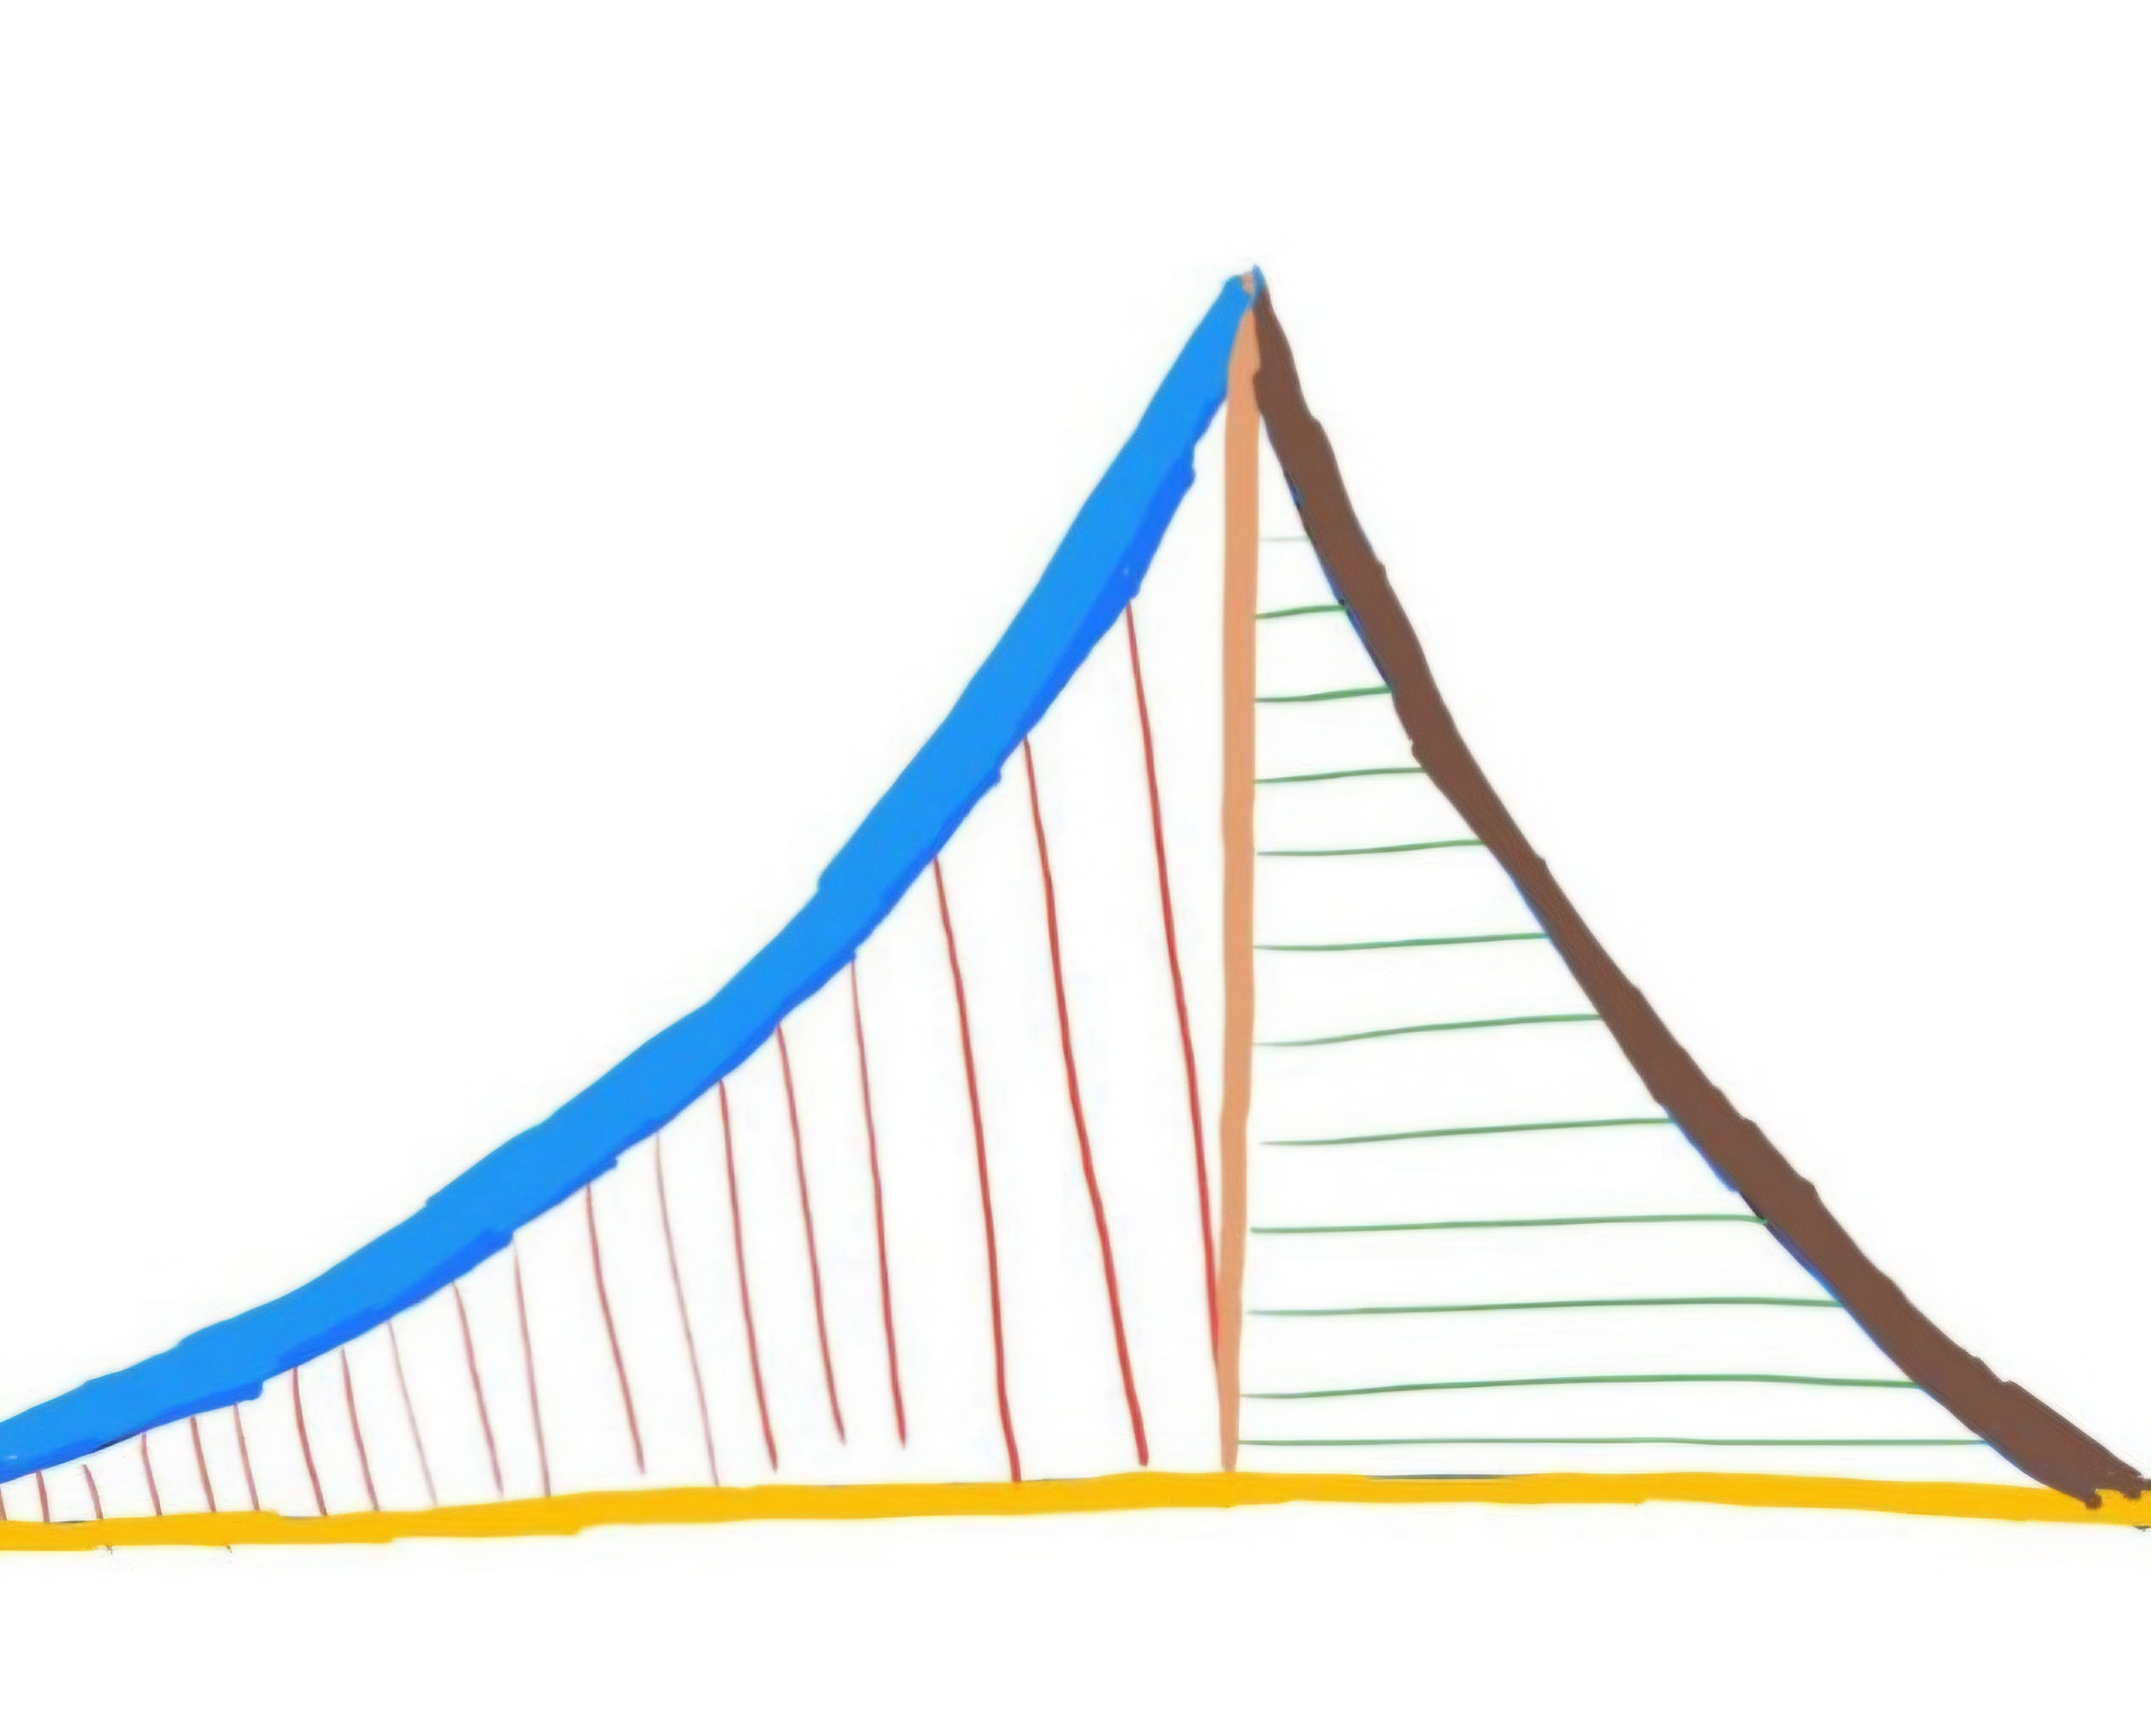
\includegraphics[width=0.2\columnwidth]{figs/logo.jpg}
\\
		{\huge	G. V. V. Sharma}\\Associate Professor,\\Department of Electrical Engineering, \\ IIT Hyderabad
	\end{center}
	%\end{flushleft}
%\IEEEpubid{\makebox[\columnwidth]{978-1-7281-5966-1/20/\$31.00 ©2020 IEEE \hfill} \hspace{\columnsep}\makebox[\columnwidth]{ }}
}
\maketitle

\newpage
\section*{About this Book}

This book introduces C programming for middle school children based on the
 NCERT mathematics textbook of Class 7.  

There is no copyright, so readers are free to print and share.  

This book is dedicated to my Hindi teacher in middle school, Shri Mandavi.
\begin{flushright}
\today
\end{flushright}
Github: https://github.com/gadepall/cprog
		\\
License: https://creativecommons.org/licenses/by-sa/3.0/
\\
and
\\
https://www.gnu.org/licenses/fdl-1.3.en.html

\newpage


\tableofcontents

\newpage
%\twocolumn
\onecolumn


%\renewcommand{\theequation}{\theenumi}
\numberwithin{equation}{enumi}
%\numberwithin{figure}{enumi}
%\numberwithin{figure}{section}
%\numberwithin{figure}{subsection}
\renewcommand{\thefigure}{\theenumi}
\renewcommand{\thetable}{\theenumi}

\section{Integers}
\subsection{Formulae}
\begin{enumerate}[label=\thesubsection.\arabic*, ref=\thesubsection.\theenumi]
\item Do the following addition through a C program
	$$17+23$$
	\\
	\solution
	\lstinputlisting{codes/integer/add.c}
\item Do the following subtraction through a C program
$$7-9$$
	\\
	\solution
	\lstinputlisting{codes/integer/sub.c}
\item Mulitply the following through a C program
	$$4\times \brak{-8}$$
	\\
	\solution
	\lstinputlisting{codes/integer/mul.c}
\item Perform the following division
	$$\brak{-100}\div 5$$
	\\
	\solution
	\lstinputlisting{codes/integer/div.c}
\end{enumerate}

\subsection{NCERT}
\begin{enumerate}[label=\thesubsection.\arabic*, ref=\thesubsection.\theenumi]
\item Do the following addition through a C program
	$$17+23$$
	\\
	\solution
	\lstinputlisting{codes/add.c}
\item Do the following subtraction through a C program
$$7-9$$
	\\
	\solution
	\lstinputlisting{codes/sub.c}
\item Mulitply the following through a C program
	$$4\times \brak{-8}$$
	\\
	\solution
	\lstinputlisting{codes/mul.c}
\item Perform the following division
	$$\brak{-100}\div 5$$
	\\
	\solution
	\lstinputlisting{codes/div.c}
\end{enumerate}
Compute the following
\begin{enumerate}[label=\thesubsection.\arabic*, ref=\thesubsection.\theenumi,resume*]
	\begin{multicols}{4}
\item $\brak{-75}+18$
\item $19+\brak{-25}$
\item $27+\brak{-27}$
\item $\brak{-20}+0$
\item $\brak{-35}+\brak{-10}$
\item $\brak{-10}+3$
\item $17-(-21)$
\item $8\times(-2)$
\item $3\times(-7)$
\item $10\times(-1)$
\item $6\times(-19)$
\item $12\times(-32)$
\item $7\times(-22)$
\item $15\times(-16)$
\item $21\times(-32)$
\item $(-42)\times 12$
\item $(-55)\times 15$
\item $(-5)\times \brak{-6}$
\item $\brak{-6}\times(-7)$
\item $3\times(-1)$
\item $\brak{-1}\times 225$
\item $\brak{-21}\times(-30)$
\item $\brak{-316}\times(-1)$
\item	$\brak{-81}\div 9$
\item	$\brak{-75}\div 5$
\item	$\brak{-32}\div 2$
\item	$125\div \brak{-25}$
\item	$80\div \brak{-5}$
\item	$64\div \brak{-16}$
\item	$\brak{-30}\div 10$
\item	$50\div \brak{-5}$
\item	$\brak{-36}\div \brak{-9}$
\item	$\brak{-49}\div \brak{-49}$
\end{multicols}
\end{enumerate}
\begin{enumerate}[label=\thesubsection.\arabic*, ref=\thesubsection.\theenumi,resume*]
	\begin{multicols}{2}
\item	$13\div \sbrak{\brak{-2}+1}$
\item	$\brak{-31}\div \sbrak{\brak{-30}+\brak{-1}}$
\item	$\sbrak{\brak{-36}\div 12}\div \brak{3}$
\item	$\sbrak{\brak{-6}+5}\div \sbrak{\brak{-2}+1}$
	\end{multicols}
\end{enumerate}
Fill in the blanks
\begin{enumerate}[label=\thesubsection.\arabic*, ref=\thesubsection.\theenumi,resume*]
	\begin{multicols}{2}
		\item	$20 \div \rule{1cm}{0.1pt}=-2$
		\item	$\rule{1cm}{0.1pt}\div 4=-3$
	\end{multicols}
\end{enumerate}
\begin{enumerate}[label=\thesubsection.\arabic*, ref=\thesubsection.\theenumi,resume*]
	\item In a test (+5) marks are given for every correct answer and (-2) marks for every incorrect answer.  
		\begin{enumerate}
			\item Radhika answered all the questions and scored 30 marks though she got 10 correct answers.
			\item Jay also answered al the questions and scored (-12) marks though he got 4 correct answers.  How many incorrect answers had they  attempted?
		\end{enumerate}
	\item A shopkeeper earns a profit of \rupee 1 by selling one pen and incurs a loss of 40 paise per pencil while selling pencils of her old stock.  
		\begin{enumerate}
			\item In a particular month she incurs a loss of \rupee 5.  In this period she sold 45 pens.  How many pencils did she sell in this period?
			\item In the next month she earns neither profit nor loss.  If she sold 70 pens, how many pencils did she sell?
			\item The temperature at 12 noon was 10\degree C above zero. If it decreases at the rate of 2\degree C per hour unitl midnight, at what time would the temperature be 8\degree C below zero? 
	\item In a class test (+3) marks are given for every correct answer and (-2) marks for every incorrect answer and no marks for not attempting any question.   
		\begin{enumerate}
			\item Radhika scored 20 marks.  If she got 12 correct answers, how many questions has she attempted incorrectly?
			\item Mohini scores -5 marks in this test, though she has got 7 correct answers.   How many questions has she attempted incorrectly?
		\end{enumerate}
	\item An elevator descends a mine shaft at the rate of $6m/min$.  If the descent starts from $10m$ above the ground, how long will it take to reach $-350m$.
		\end{enumerate}
\end{enumerate}

\section{Decimal Numbers}
\subsection{Formulae}
Find
\begin{enumerate}[label=\thesubsection.\arabic*,ref=\thesubsection.\theenumi,itemsep=1ex]
	\item $\frac{5}{3}+\frac{3}{5}$
		\\
		\solution
	\lstinputlisting{codes/deci/add.c}
	\item $\frac{2}{3}-\frac{3}{7}$
		\\
		\solution
	\lstinputlisting{codes/deci/sub.c}
	\item $5.6\times 1.4$
		\\
		\solution
	\lstinputlisting{codes/deci/mul.c}
	\item $ 37.8\div 1.4$
		\\
		\solution
	\lstinputlisting{codes/deci/div.c}
\end{enumerate}

\subsection{NCERT}
Find
\begin{enumerate}[label=\thesection.\arabic*,ref=\thesection.\theenumi,itemsep=1ex]
	\item $\frac{5}{3}+\frac{3}{5}$
		\\
		\solution
	\lstinputlisting{codes/deci/add.c}
	\item $\frac{2}{3}-\frac{3}{7}$
		\\
		\solution
	\lstinputlisting{codes/deci/sub.c}
	\item $5.6\times 1.4$
		\\
		\solution
	\lstinputlisting{codes/deci/mul.c}
	\item $ 37.8\div 1.4$
		\\
		\solution
	\lstinputlisting{codes/deci/div.c}
\end{enumerate}
Find
\begin{enumerate}[label=\thesection.\arabic*,ref=\thesection.\theenumi,itemsep=1ex,resume*]
	\begin{multicols}{4}
%
	\item $\frac{2}{7}\times 3$
	\item $\frac{9}{7}\times 6$
	\item $\frac{1}{8}\times 3$
	\item $\frac{13}{11}\times 6$
	\item $\frac{2}{5}\times 2$
	\item $3\times 5\frac{1}{5}$
	\item $5\times 6\frac{3}{4}$
	\item $7\times 2\frac{1}{4}$
	\item $4\times 6\frac{1}{3}$
	\item $6\times 3\frac{1}{4}$
	\item $8\times 3\frac{2}{5}$
	\item $\frac{1}{2}\times \frac{1}{7}$
	\item $\frac{1}{5}\times \frac{1}{7}$
	\item $\frac{1}{3}\times \frac{4}{5}$
	\item $\frac{2}{3}\times \frac{1}{5}$
	\item $\frac{8}{3}\times \frac{4}{7}$
	\item $\frac{3}{4}\times \frac{2}{3}$
	\item $\frac{2}{3}\times 2\frac{2}{3}$
	\item $\frac{2}{7}\times \frac{7}{9}$
	\item $\frac{3}{8}\times \frac{6}{4}$
	\item $\frac{9}{5}\times \frac{3}{5}$
	\item $\frac{1}{3}\times \frac{15}{8}$
	\item $\frac{11}{2}\times \frac{3}{10}$
	\item $\frac{4}{5}\times \frac{12}{7}$
	\item $\frac{2}{5}\times 5\frac{1}{4}$
	\item $6\frac{2}{5}\times \frac{7}{9}$
	\item $\frac{3}{2}\times 5\frac{1}{3}$
	\item $\frac{5}{6}\times 2\frac{3}{7}$
	\item $3\frac{2}{5}\times \frac{4}{7}$
	\item $2\frac{3}{5}\times 3$
	\item $3\frac{4}{7}\times \frac{3}{5}$
	\item $\frac{2}{3}\times \rule{0.5cm}{0.1pt}=\frac{10}{30}$
	\item $\frac{3}{5}\times \rule{0.5cm}{0.1pt}=\frac{24}{75}$
	\item $7 \div \frac{2}{5}$
	\item $6 \div \frac{4}{7}$
	\item $2 \div \frac{8}{9}$
	\item $\frac{3}{5} \div \frac{1}{2}$
	\item $\frac{1}{2} \div \frac{3}{5}$
	\item $2\frac{1}{2} \div \frac{3}{5}$
	\item $5\frac{1}{6} \div \frac{9}{2}$
	\item $12 \div \frac{3}{4}$
	\item $14 \div \frac{5}{6}$
	\item $8 \div \frac{7}{3}$
	\item $4 \div \frac{8}{3}$
	\item $3 \div 2\frac{1}{3}$
	\item $5 \div 3\frac{4}{7}$
	\item $\frac{7}{3}\div 2$
	\item $\frac{4}{9}\div 5$ 
	\item $\frac{6}{13}\div 7$
	\item $4\frac{1}{3}\div 3$
	\item $3\frac{1}{2}\div 4$
	\item $4\frac{3}{7}\div 7$
	\item $\frac{2}{5} \div \frac{1}{2}$
	\item $\frac{4}{9} \div \frac{2}{3}$
	\item $\frac{3}{7} \div \frac{8}{7}$
	\item $2\frac{1}{3} \div \frac{3}{5}$
	\item $3\frac{1}{2} \div \frac{8}{3}$
	\item $\frac{2}{5} \div 1\frac{1}{2}$
	\item $3\frac{1}{5} \div 1\frac{2}{3}$
	\item $2\frac{1}{5} \div 1\frac{1}{5}$
	\item $0.2\times 6$
	\item $8\times 4.6$
	\item $2.71\times 5$
	\item $20.1\times 4$
	\item $0.05\times 7$
	\item $211.02\times 4$
	\item $2\times 0.86$
	\item $2.5\times 0.3$
	\item $0.1\times 51.7$
	\item $0.2\times 316.8$
	\item $1.3\times 3.1$
	\item $0.5\times 0.05$
	\item $11.2\times 0.15$
	\item $1.07\times 0.02$
	\item $10.05\times 1.05$
	\item $101.01\times 0.01$
	\item $100.01\times 1.1$
	\item $7.75\times 0.25$
	\item $42.8\times 0.02$
	\item $0.4 \div  2$
	\item $0.35 \div  5$
	\item $2.48 \div  4$
	\item $65.4 \div  6$
	\item $651.2 \div  4$
	\item $14.49 \div  7$
	\item $3.96  \div  4$
	\item $0.80 \div  5$
	\item $7 \div 3.5$
	\item $ 36\div 0.2$
	\item $3.25 \div 0.5$
	\item $ 30.94\div 0.7$
	\item $ 0.5\div 0.25$
	\item $ 7.75\div 0.25$
	\item $ 76.5\div 0.15$
	\item $ 2.73\div 1.3$
	\item $\frac{5}{4}+\frac{-11}{4}$
	\item $\frac{-9}{10}+\frac{22}{15}$
	\item $\frac{-3}{-11}+\frac{5}{9}$
	\item $\frac{-8}{19}+\frac{-2}{57}$
	\item $\frac{-2}{3}+{0}$
	\item $\frac{-13}{7}+\frac{6}{7}$
	\item $\frac{19}{5}+\frac{-7}{5}$
	\item $\frac{-5}{6}+\frac{-3}{11}$
	\item $-2\frac{1}{3}+4\frac{3}{5}$
	\item $\frac{7}{24}-\frac{17}{36}$
	\item $\frac{5}{63}-\frac{-6}{21}$
	\item $\frac{-6}{13}-\frac{-7}{15}$
	\item $\frac{-3}{8}-\frac{7}{11}$
	\item $-2\frac{1}{9}-{6}$
	\item $\frac{7}{9}-\frac{2}{5}$
	\item $2\frac{1}{5}-\frac{-1}{3}$
	\item $\frac{9}{2}\times \frac{-7}{4}$
	\item $\frac{3}{10}\times {-9}$
	\item $\frac{-6}{5}\times \frac{9}{11}$
	\item $\frac{3}{7}\times \frac{-2}{5}$
	\item $\frac{3}{11}\times \frac{2}{5}$
	\item $\frac{3}{-5}\times \frac{-5}{3}$
	\item ${-4}\div \frac{2}{3}$
	\item $\frac{-3}{5}\div {2}$
	\item $\frac{-4}{5}\div {-3}$
	\item $\frac{-1}{8}\div \frac{3}{4}$
	\item $\frac{-2}{13}\div \frac{1}{7}$
	\item $\frac{-7}{12}\div \frac{-2}{13}$
	\item $\frac{3}{13}\div \frac{-4}{65}$
	\item $\frac{-3}{5}\times 7\frac{}{}$
	\item $\frac{-6}{5}\times -2\frac{}{}$
	\item $\frac{-3}{4}\times \frac{1}{7}$
	\item $\frac{2}{3}\times \frac{-5}{9}$
	\item $\frac{2}{3}\times \frac{-7}{8}$
	\item $\frac{-6}{7}\times \frac{5}{7}$
	\end{multicols}
\end{enumerate}
Find
\begin{enumerate}[label=\thesection.\arabic*,ref=\thesection.\theenumi,resume*,itemsep=1ex]
	\begin{multicols}{2}
	\item $\frac{1}{2}$ of
		\begin{enumerate}
			\item $2\frac{3}{4}$
			\item $4\frac{2}{9}$
		\end{enumerate}
	\item $\frac{5}{8}$ of
		\begin{enumerate}
			\item $3\frac{5}{6}$
			\item $9\frac{2}{3}$
		\end{enumerate}
	\end{multicols}
\end{enumerate}
Find
\begin{enumerate}[label=\thesection.\arabic*,ref=\thesection.\theenumi,resume*]
	\begin{multicols}{2}
	\item $\frac{1}{4}$ of
		\begin{enumerate}
			\item $\frac{1}{4}$
			\item $\frac{3}{5}$
			\item $\frac{4}{3}$
		\end{enumerate}
	\item $\frac{1}{7}$ of
		\begin{enumerate}
			\item $\frac{2}{9}$
			\item $\frac{6}{5}$
			\item $\frac{3}{10}$
		\end{enumerate}
	\end{multicols}
\end{enumerate}
\begin{enumerate}[label=\thesection.\arabic*,ref=\thesection.\theenumi,resume*]
	\item  In a class of 40 students $\frac{1}{5}$ of the total number of students like to study English, 
$\frac{2}{5}$ of the total number like to study Mathematics and the remaining students like to study Science.
\begin{enumerate}
	\item How many students like to study English?
	\item How many students like to study Mathematics?
	\item How many students like to study Science?
\end{enumerate}
\item Vidya and Pratap went for a picnic.  Their mother gave them a water bottle that contained 5 litres of water.  Vidya consumed $\frac{2}{5}$ of the water.  Pratap consumed the remaining water.
	\begin{enumerate}
		\item How much water did Vidya drink?
		\item What fraction of the total quantity of water did Pratap drink?
	\end{enumerate}
\item Shaili plants 4 saplings in a row, in her garden.  The distance between two adjacent saplings is $\frac{3}{4}m$. Find the distance between the first and the last sapling.
\item Lipika reads a book for $1\frac{3}{4}$ hours everyday.  She reads the entire book in 6 days.  How many hours in all were required by her to read the book.
\item A car runs $16km$ using 1 litre of petrol.  How much distance will it cover using $2\frac{3}{4}$ litres of petrol.
\item The side of an equilateral triangle is $3.5cm$.  Find its perimeter.  
\item The length of a rectangle is $7.1cm$ and its breadth is $2.5cm$.  What is its area?
\item Find the area of a rectangle whose length is $5.7cm$ and breadth is $3cm$. 
\item A two wheeler covers a distance of $55.3km$ in one litre of petrol.  How much will it cover in 10 litres of petrol?
\item Savita was preparing a design to decorate her classroom.  She needed a few coloured strips of paper of length $1.9cm$ each.  She had a strip of coloured paper of length $9.5cm$.  How many pieces of the required length will she get out of this strip? 
\item Each side of a regular polygon is $2.5cm$ in length.  The perimeter of the polygon is $12.5cm$.  How many sides does the polygon have?
\item A car covers a distance of $89.1km$ in $2.2$ hours.  What is the average distance covered by it in 1 hour?
\item A vehicle covers a distance of $43.2km$ in in $2.4$ litres of petrol.  How much will it cover in one litre of petrol?
\item 
	A collection of 10 chips with different colours is given in 
\figref{fig:percent2}.
Fill the table 
and find the percentage of chips of each colour.
\begin{figure}[H]
  \centering
  \begin{subfigure}{0.4\textwidth}
    
\includegraphics[width=\textwidth]{figs/percent2.jpg}
    \caption{Chips}
  \end{subfigure}
  \hfill
  \begin{subfigure}{0.4\textwidth}
    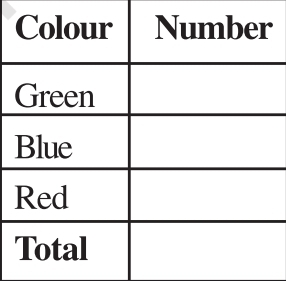
\includegraphics[width=\textwidth]{figs/percent3.jpg}
    \caption{Table}
  \end{subfigure}
  \caption{}
  \label{fig:percent2}
\end{figure}
\item 	Mala has a collection of bangles. She has 20 gold bangles and 10 silver bangles. What is the percentage of bangles of each type? Can you put it in the tabular form?
\item 	Out of 25 children in a class, 15 are girls. What is the percentage of girls?
\item Out of 32 students, 8 are absent. What per cent of the students are absent? 
\item There are 25 radios, 16 of them are out of order. What per cent of radios are out of order?
\item  A shop has 500 items, out of which 5 are defective. What per cent are defective? 
\item  There are 120 voters, 90 of them voted yes. What per cent voted yes?
\item 	A survey of 40 children showed that 25\% liked playing football. How many children liked playing football?
\item	Rahul bought a sweater and saved  \rupee 200 when a discount of 25\% was given. What was the price of the sweater before the discount?
\item 	9 is 25\% of what number? 
\item 	75\% of what number is 15?
\item Out of 15,000 voters in a constituency, 60\% voted. Find the percentage of voters who did not vote. Can you now find how many actually did not vote?
\item  Meeta saves \rupee 4000 from her salary. If this is 10\% of her salary. What is her salary?
\item  A local cricket team played 20
	matches in one season. It won 25\% of them. How many matches did they win?
\item Reena’s mother said, to make idlis, you must take two parts rice and one part urad dal. What percentage of such a mixture would be rice and what percentage would be urad dal?
\item If \rupee 250 is to be divided amongst Ravi, Raju and Roy, so that Ravi gets two parts, Raju three parts and Roy five parts. How much money will each get? What will it be in percentages?
\item 	Divide 15 sweets between Manu and Sonu so that they get 20 \% and 80 \% of them respectively.
\item If angles of a triangle are in the ratio 2 : 3 : 4. Find the value of each angle.
\item A school team won 6 games this year against 4 games won last year. What is the per cent increase?
\item The number of illiterate persons in a country decreased from 150 lakhs to 100 lakhs in 10 years. What is the percentage of decrease?
\item Find Percentage of increase or decrease
	\begin{enumerate}
	\item  Price of shirt decreased from \rupee 280 to \rupee 210.
	\item Marks in a test increased from 20 to 30.
	\end{enumerate}
\item  My mother says, in her childhood petrol was \rupee 1 a litre. It is \rupee 52 per litre today. By what Percentage has the price gone up?
\item The cost of a flower vase is \rupee 120. If the shopkeeper sells it at a loss of 10\%, find the price at which it is sold.
\item Selling price of a toy car is \rupee 540. If the profit made by shopkeeper is 20\%, what is the cost price of this toy?
\item A shopkeeper bought a chair for \rupee 375 and sold it for \rupee 400. Find the gain Percentage. 
\item  Cost of an item is \rupee 50. It was sold with a profit of 12\%. Find the selling price. 
\item  An article was sold for \rupee 250 with a profit of 5\%. What was its cost price? 
\item  An item was sold for \rupee 540 at a loss of 5\%. What was its cost price?
\item Anita takes a loan of \rupee 5,000 at 15\% per year as rate of interest. Find the interest she has to pay at the end of one year.
\item \rupee 10,000 is invested at 5\% interest rate p.a. Find the interest at the end of one year.
\item  \rupee 3,500 is given at 7\% p.a. rate of interest. Find the interest which will be received at the end of two years.
\item  \rupee 6,050 is borrowed at 6.5\% rate of interest p.a.. Find the interest and the amount to be paid at the end of 3 years.
\item  \rupee 7,000 is borrowed at 3.5\% rate of interest p.a. borrowed for 2 years. Find the amount to be paid at the end of the second year.
\item If Manohar pays an interest of \rupee 750 for 2 years on a sum of \rupee 4,500, find the rate of interest.
\item You have \rupee 2,400 in your account and the interest rate is 5\%. After how many years would you earn \rupee 240 as interest.
\item On a certain sum the interest paid after 3 years is \rupee 450 at 5\% rate of interest per annum. Find the sum.
\item Tell what is the profit or loss in the following transactions. Also find profit per cent or loss per cent in each case. 
	\begin{enumerate}
\item  Gardening shears bought for \rupee 250 and sold for \rupee 325. 
\item  A refrigerater bought for \rupee 12,000 and sold at \rupee 13,500. 
\item  A cupboard bought for \rupee 2,500 and sold at \rupee 3,000. 
\item  A skirt bought for \rupee 250 and sold at \rupee 150.
	\end{enumerate}
\item Convert each part of the ratio to percentage
	\begin{enumerate}
		\item  3 : 1
		\item  2 : 3 : 5 
		\item  1:4 
		\item  1 : 2 : 5
	\end{enumerate}
\item  The population of a city decreased from 25,000 to 24,500. Find the percentage decrease.
\item  Arun bought a car for \rupee 3,50,000. The next year, the price went upto \rupee 3,70,000. What was the Percentage of price increase?
\item  I buy a T.V. for \rupee 10,000 and sell it at a profit of 20\%. How much money do I get for it?
\item  Juhi sells a washing machine for \rupee 13,500. She loses 20\% in the bargain. What was the price at which she bought it?
\item 
	\begin{enumerate}
		\item Chalk contains calcium, carbon and oxygen in the ratio 10:3:12. Find the percentage of carbon in chalk.
		\item  If in a stick of chalk, carbon is 3g, what is the weight of the chalk stick?
	\end{enumerate}
\item Aamani buys a book for \rupee 275 and sells it at a loss of 15\%. How much does she sell it for?
\item  Find the amount to be paid at the end of 3 years in each case
	\begin{enumerate}
\item  Principal = \rupee 1,200 at 12\% p.a.
\item  Principal = \rupee 7,500 at 5\% p.a.
	\end{enumerate}
\item  What rate gives \rupee 280 as interest on a sum of \rupee 56,000 in 2 years? 
\item  If Meena gives an interest of \rupee 45 for one year at 9\% rate p.a.. What is the sum she has borrowed?
\item	Find the missing values
	in
\figref{fig:area}
	\begin{figure}[H]
  \centering
  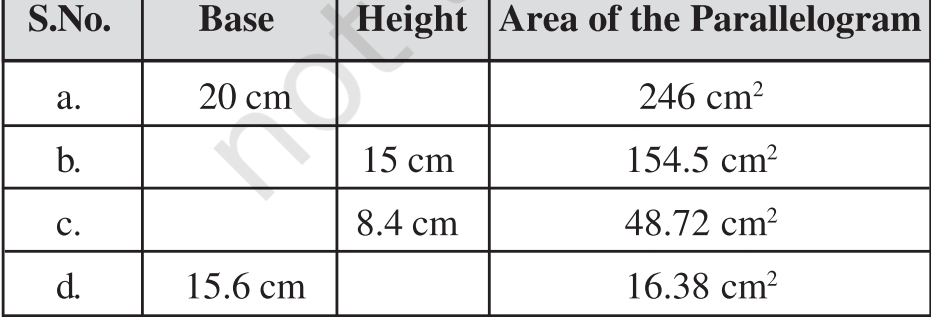
\includegraphics[width=\columnwidth]{figs/area.jpg}
  \caption{}
  \label{fig:area}
\end{figure}
\item	Find the missing values
	in
\figref{fig:area1}
	\begin{figure}[H]
  \centering
  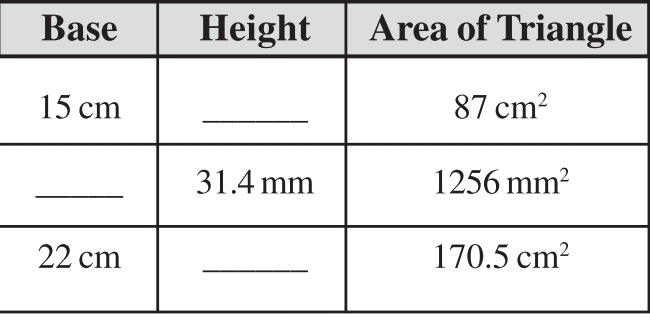
\includegraphics[width=\columnwidth]{figs/area1.jpg}
  \caption{}
  \label{fig:area1}
\end{figure}
\end{enumerate}

\section{Programming}
In a quiz, team A scored $a_1 = -40, a_2=10, a_3=0$ and team B scored $b_1=10, b_2=0, b_3=-40$ in three successive rounds.
\begin{enumerate}[label=\thesection.\arabic*, ref=\thesubsection.\theenumi]
\item  If the total scores are 
	\begin{align}
		a &= a_1+a_2+a_3
		\\
		b &= b_1+b_2+b_3
	\end{align}
	which team scored more? 
	\\
	\solution 
	\lstinputlisting{codes/prog/ifelse.c}
\item Write a function to compare the final scores.  Check for the cases when $a = -40, b = -40; a = 30, b = 20; a = -20, b = -10$.
	\\
	\solution 
	\lstinputlisting{codes/prog/func.c}
\item Use arrays and a for loop to evaluate 
	\begin{align}
		a &= \sum_{i=0}^{2}a_i
		\\
		b &= \sum_{i=0}^{2}b_i
	\end{align}
	\\
	\solution 
	\lstinputlisting{codes/prog/loop.c}
\item Revise the above code using only functions.
	\\
	\solution 
	\lstinputlisting{codes/prog/loopfunc.c}
\item Use files for the input data.
	\\
	\solution 
	\lstinputlisting{codes/prog/files.c}
\item Revise the files program using pointer arrays
	\\
	\solution 
	\lstinputlisting{codes/prog/pointer.c}
\item Revise the files program using only functions
	\\
	\solution 
	\lstinputlisting{codes/prog/filesfunc.c}
\end{enumerate}
Use ifelse  for the following
\begin{enumerate}[label=\thesection.\arabic*, ref=\thesubsection.\theenumi,resume*]
	\begin{multicols}{2}
	\item $25 \times \brak{-21} = \brak{-21}\times 25 $
	\item $\brak{-48}\div\brak{8} = 48 \div \brak{-8}$
	\item $\brak{-23}\times  20 = 23 \times \brak{-20}$
	\item $90 \div \brak{-45} = \brak{-90}\div 45$
	\item $ \brak{-136}\div 4=136 \div \brak{-4} $
	\item $10\times  \sbrak{6+\brak{-2}} =10\times 6+10 \times \brak{-2} $
	\item $10\times  \sbrak{6-\brak{-2}} =10\times 6-10 \times \brak{-2} $
	\item $\brak{-15}\times  \sbrak{\brak{-7}-\brak{-1}} =\brak{-15}\times\brak{-7}-\brak{-15} \times \brak{-1} $
	\item $18\times  \sbrak{\brak{7}+\brak{-3}} =18\times\brak{7}+18 \times \brak{-3} $
	\item $\brak{-21}\times  \sbrak{\brak{-4}+\brak{-6}} =\brak{-21}\times\brak{-4}+\brak{-21} \times \brak{-6} $
	\item $\brak{-15}\times  \sbrak{\brak{-7}+\brak{-1}} =\brak{-15}\times\brak{-7}+\brak{-15} \times \brak{-1} $
\item $10\times 10^{11} = 100^{11}$
\item $2^{3} > 5^{2}$
\item $2^3\times 3^{2} = 6^{5}$
\item $3^0 = 1000^{0}$
\end{multicols}
	\item 		An angle is greater than 45\degree. Is its complementary angle greater than 45\degree or equal to 45\degree or less than 45\degree?
	\item Is there a triangle whose sides have lengths $10.2 cm, 5.8 cm$ and $4.5 cm$?
\item		The lengths of two sides of a triangle are $6 cm$ and $8 cm$. Between which two numbers can length of the third side fall?
\item	Is it possible to have a triangle with the following sides? 
	\begin{enumerate}
		\begin{multicols}{3}
\item $2 cm, 3 cm, 5 cm $ 
\item $3 cm, 6 cm, 7 cm $
\item $ 6 cm, 3 cm, 2 cm$
\end{multicols}
	\end{enumerate}
\item 	The lengths of two sides of a triangle are $12 cm$ and $15 cm$. Between what two measures should the length of the third side fall?
\end{enumerate}
Which is greater?
\begin{enumerate}[label=\thesection.\arabic*, ref=\thesubsection.\theenumi,resume*,itemsep=1ex]
	\begin{multicols}{2}
	\item $\frac{1}{2}$ of $\frac{3}{4}$
	or $\frac{3}{5}$ of $\frac{5}{8}$
	\item $\frac{1}{2}$ of $\frac{6}{7}$
	or $\frac{2}{3}$ of $\frac{3}{7}$
\end{multicols}
\end{enumerate}
Use arrays for the following
\begin{enumerate}[label=\thesection.\arabic*, ref=\thesubsection.\theenumi,resume*]
	\begin{multicols}{2}
	\item $\brak{-12}\times  \brak{-11}\times \brak{10} $
	\item $\brak{9}\times\brak{-3} \times \brak{-6}$ 
	\item $\brak{-18}\times\brak{-5} \times \brak{-4}$ 
	\item $\brak{-3}\times\brak{-6} \times \brak{-2} \times \brak{-1}$ 
\end{multicols}
\end{enumerate}
Use recursion for the following
\begin{enumerate}[label=\thesection.\arabic*, ref=\thesubsection.\theenumi,resume*]
	\item $\brak{-1}\times\brak{-2} \times \brak{-3} \times \brak{-4}$ 
\end{enumerate}
Use matrices for the following
\begin{enumerate}[label=\thesection.\arabic*, ref=\thesubsection.\theenumi,resume*]
	\item The difference in the measures of two complementary angles is 12\degree. Find the measures of the angles.
\item Among two supplementary angles the measure of the larger angle is $44\degree$  more than the measure of the smaller. Find their measures
\end{enumerate}
Identify which of the following pairs of angles are complementary and which are supplementary.
\begin{enumerate}[label=\thesection.\arabic*, ref=\thesubsection.\theenumi,resume*]
	\begin{multicols}{4}
	\item  65\degree, 115\degree
	\item  63\degree, 27\degree 
	\item  130\degree, 50\degree 
	\item 45\degree, 45\degree 
	\item  112\degree, 68\degree 
	\item  80\degree, 10\degree
\end{multicols}
\end{enumerate}
Which of these are negative rational numbers?
\begin{enumerate}[label=\thesection.\arabic*, ref=\thesubsection.\theenumi,resume*,itemsep=1ex]
	\begin{multicols}{4}
	\item $\frac{-2}{3}$
	\item $\frac{5}{7}$
	\item $\frac{3}{-5}$
	\item $\frac{6}{11}$
	\item $\frac{-2}{-9}$
	\item 0
\end{multicols}
\end{enumerate}
Reduce to standard form
\begin{enumerate}[label=\thesection.\arabic*, ref=\thesubsection.\theenumi,resume*,itemsep=1ex]
	\begin{multicols}{4}
	\item $\frac{-45}{30}$
	\item $\frac{36}{-24}$
	\item $\frac{-3}{-15}$
	\item $\frac{-18}{45}$
	\item $\frac{-12}{18}$
	\item $\frac{-8}{6}$
	\item $\frac{25}{45}$
	\item $\frac{-44}{72}$
	\item $\frac{-8}{10}$
\end{multicols}
\end{enumerate}
Compare the following and fill in the blanks
\begin{enumerate}[label=\thesection.\arabic*, ref=\thesubsection.\theenumi,resume*,itemsep=1ex]
	\begin{multicols}{4}
		\item $\frac{-5}{7} \rule{0.5cm}{0.1pt} \frac{2}{3}$
		\item $\frac{-8}{5} \rule{0.5cm}{0.1pt} \frac{-7}{4}$
		\item ${0} \rule{0.5cm}{0.1pt} \frac{-7}{6}$
		\item $\frac{-4}{5} \rule{0.5cm}{0.1pt} \frac{-5}{7}$
		\item $\frac{1}{-3} \rule{0.5cm}{0.1pt} \frac{-1}{4}$
		\item $\frac{-7}{8} \rule{0.5cm}{0.1pt} \frac{14}{-16}$
		\item $\frac{5}{-11} \rule{0.5cm}{0.1pt} \frac{-5}{11}$
		\item $\frac{2}{3} \rule{0.5cm}{0.1pt} \frac{5}{7}$
		\item $\frac{-3}{8} \rule{0.5cm}{0.1pt} \frac{-2}{7}$
		\item $\frac{-4}{3} \rule{0.5cm}{0.1pt} \frac{-3}{2}$
		\item $\frac{-7}{21} \rule{0.5cm}{0.1pt} \frac{3}{9}$
		\item $\frac{-3}{5} \rule{0.5cm}{0.1pt} \frac{-12}{20}$
		\item $\frac{-5}{-9} \rule{0.5cm}{0.1pt} \frac{5}{-9}$
		\item $\frac{-16}{20} \rule{0.5cm}{0.1pt} \frac{20}{-25}$
		\item $\frac{8}{-5} \rule{0.5cm}{0.1pt} \frac{-24}{15}$
		\item $\frac{-2}{-3} \rule{0.5cm}{0.1pt} \frac{2}{3}$
		\item $\frac{1}{3} \rule{0.5cm}{0.1pt} \frac{-1}{9}$
		\item $\frac{4}{-9} \rule{0.5cm}{0.1pt} \frac{-16}{36}$
		\item $\frac{2}{3} \rule{0.5cm}{0.1pt} \frac{5}{2}$
		\item $\frac{-1}{4} \rule{0.5cm}{0.1pt} \frac{1}{4}$
		\item $\frac{-5}{6} \rule{0.5cm}{0.1pt} \frac{-4}{3}$
		\item $-3\frac{2}{7} \rule{0.5cm}{0.1pt} -3\frac{4}{5}$
		\item $\frac{-3}{4} \rule{0.5cm}{0.1pt} \frac{2}{-3}$
\end{multicols}
\end{enumerate}
		Write four more numbers in the following pattern
\begin{enumerate}[label=\thesection.\arabic*, ref=\thesection.\theenumi,resume*,itemsep=1ex]
	\begin{multicols}{3}
	\item $\frac{-1}{3},\frac{-2}{6},\frac{-3}{9},\frac{-4}{12}$
	\item $\frac{-3}{5},\frac{-6}{10},\frac{-9}{15},\frac{-12}{20}$
	\item $\frac{-1}{4},\frac{-2}{8},\frac{-3}{12}$
	\item $\frac{-1}{6},\frac{2}{-12},\frac{3}{-18},\frac{4}{-24}$
	\item $\frac{-2}{3},\frac{2}{-3},\frac{4}{-6},\frac{6}{-9}$
\end{multicols}
		\end{enumerate}

\section{Data Handling}
\begin{enumerate}[label=\thesection.\arabic*, ref=\thesection.\theenumi]
\item Find
	\begin{enumerate}
	\begin{multicols}{3}
	\item $2.7\times 4$
	\item $1.8\times 1.2$
	\item $2.3\times 4.35$
	\end{multicols}
	\end{enumerate}
and arrange the products in descending order.
\item Find the average of $4.2, 3.8$ and $7.6$.
\item Ashish studies for 4 hours, 5 hours and and 3 hours respectively on three consecutive days.  How many hours does he study daily on an average?
\item A batsman scored the following number of runs in 6 innings.  
	$$36, 35, 50, 46, 60, 55$$
	Calculate the mean runs scored by him in an inning.
\item The ages in years of 10 teachers of a school are
	$$32, 41, 28, 54, 35, 26, 23, 33, 38, 40$$
	\begin{enumerate}
		\item What is the age of the oldest teacher and that of the youngest teacher?
		\item What is the range of the ages of the teachers?
		\item What is the mean age of these teachers?
	\end{enumerate}
\item Organize the following marks in a class assessment, in tabular form with columns as marks and frequency.
	\begin{enumerate}
		\item Which number is the highest?
		\item Which number is the lowest?
		\item What is the range of the data?
		\item Find the arithmetic mean.
	\end{enumerate}
\item A cricketer scores the following runs in eight innings.
	$$58, 76, 40, 35, 46, 45, 0, 100$$
	Find the mean score.
\item Generate the following table using a C program
	\begin{figure}[H]
  \centering
  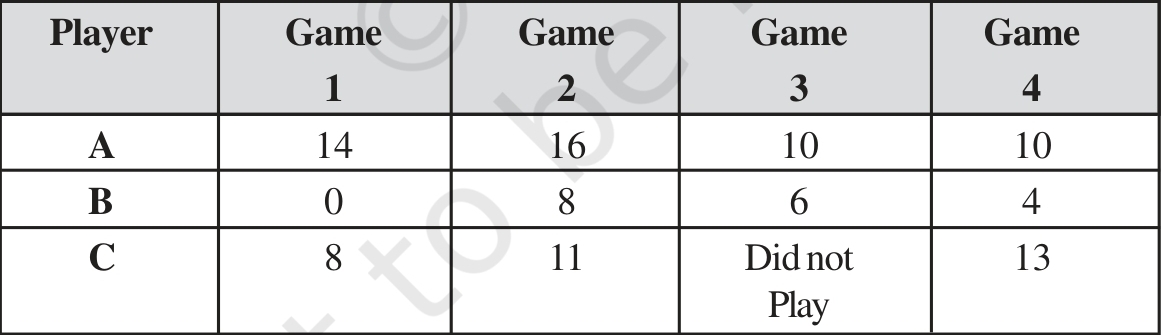
\includegraphics[width=\columnwidth]{figs/data.jpg}
  \caption{}
  \label{fig:data}
\end{figure}
and answer the following questions.
\begin{enumerate}
	\item Find the mean to determine $A's$ average number of points scored per game.
	\item Who is the best performer?
\end{enumerate}
\item The marks out of 100 obtained by a group of students in a science test are 85, 76, 90, 85, 39, 48, 56, 95, 81 and 75.  Find the 
	\begin{enumerate}
		\item Highest and lowest marks obtained by the students.
		\item Range of marks obtained.
		\item  Mean marks obtained by the group.
	\end{enumerate}
\item The enrolment in a school during six consecutive years was as follows  
	$$1555, 1670, 1750, 2013, 2540, 2820$$
	Find the mean enrolment of the school for this period.
\item The rainfall (in mm) in a city on 7 days a week was recorded as in 
  \tabref{fig:data2}.  Generate this table using a C program.
	\begin{figure}[H]
  \centering
  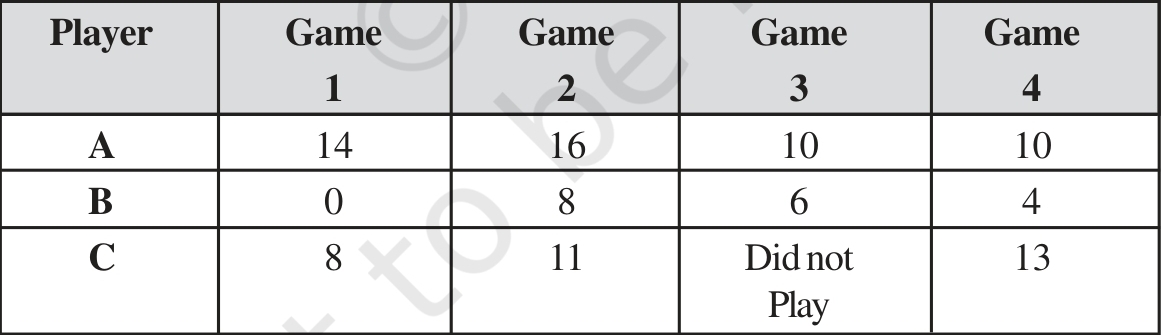
\includegraphics[width=\columnwidth]{figs/data.jpg}
  \caption{}
  \label{fig:data2}
\end{figure}
\item Find the range of the rainfall in the given data.
\item Find the mean rainfall for the week.
\item On how many days was the rainfall less than the mean rainfall 
\item The height of 10 girls was measured in cm and result was as follows
	$$135, 150, 139, 128, 151, 132, 146, 149, 143, 141.$$
	\begin{enumerate}
		\item What is the height of the tallest girl?
		\item What is the height of the shortest girl?
		\item What is the range of the data?
		\item What is the mean height of the girls?
		\item How many girls have heights more than the mean height?
	\end{enumerate}
\item To find out the weekly demand for different sizes of shirt, a shopkeeper kept records of sales of sizes as shown in 
  \eqref{fig:mode}.  This is the record for a week.  Find the mode of the data.
	\begin{figure}[H]
  \centering
  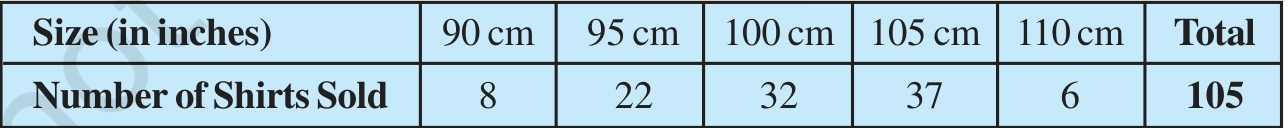
\includegraphics[width=\columnwidth]{figs/mode.jpg}
  \caption{}
  \label{fig:mode}
\end{figure}
\item Find the mode of the given set of numbers
	$$1,1,1,2,2,2,2,3,4,4$$.
\item Following are the margins of victory in the football matches of a league.  Find the mode of this data.
	\begin{gather*}
	1,3,2,5,1,4,6,2,5,2,2,2,4,1,2,3,1,1,2,3,2,6,4,3,2,
	\\
	1,1,4,2,1,5,3,3,2,3,2,42,1,2.
	\end{gather*}
\end{enumerate}
Find the mode of
\begin{enumerate}[label=\thesection.\arabic*, ref=\thesection.\theenumi]
\item 	
		2,6,5,3,0,4,3,2,4,5,2,4
\item 
%	\begin{gather}
		2,4,16,12,14,14,16,14,10,14,18,14
%	\end{gather}
\end{enumerate}

\section{Math Library}
\begin{enumerate}[label=\thesection.\arabic*, ref=\thesection.\theenumi]
\item Determine whether the triangle whose lengths of sides are $3 cm, 4 cm, 5 cm$ is a right-angled triangle.
\item $\triangle ABC$ is right-angled at $C$. If $AC = 5 cm$ and $BC = 12 cm$ find the length of $AB$.
\item $PQR$ is a triangle, right-angled at $P$. If $PQ = 10cm$ and $PR = 24 cm$, find $QR$.
\item $ABC$ is a triangle, right-angled at $C$. If $AB = 25 cm$ and $AC = 7 cm$, find $BC$.
\item A $15 m$ long ladder reached a window $12 m$ high from the ground on placing it against a wall at a distance $a$. Find the distance of the foot of the ladder from the wall.
\item  Which of the following can be the sides of a right triangle? 
\begin{enumerate}
	\item $2.5 cm,6.5 cm, 6 cm.$ 
	\item $ 2 cm, 2 cm, 5 cm.$ 
	\item $ 1.5 cm, 2cm, 2.5 cm.$
\end{enumerate}
\item A tree is broken at a height of $5 m$ from the ground and its top touches the ground at a distance of $12 m$ from the base of the tree. Find the original height of the tree.
\item Find the perimeter of the rectangle whose length is $40 cm$ and a diagonal is $41 cm$. 
\item The diagonals of a rhombus measure $16 cm$ and $30 cm$. Find its perimeter.
\item Find the values of the following expressions for $x = 2$. 
	\begin{enumerate}
\item $x + 4$
\item  $4x – 3$ 
\item  $19-5x^2$
\item  $100 – 10x^3$
	\end{enumerate}
\item Find the value of the following expressions when $n = – 2.$ 
	\begin{enumerate}
\item $5n – 2$
\item  $5n^2 + 5n – 2 $
\item  $n^3 + 5n^2 + 5n – 2$
	\end{enumerate}
\item Find the value of the following expressions for $a = 3, b = 2$. 
	\begin{enumerate}
\item $a + b$				
\item $ 7a – 4b $
\item $ a^2+2ab+b^2$
\item $ a^3 – b^3$
\end{enumerate}
\item If $m = 2$, find the value of
	\begin{enumerate}
\item $ m – 2$
\item $ 3m – 5 $
\item $ 9 – 5m $
\item $ 3m^2 – 2m – 7 $
\item $ \frac{5m^4}{ 2}$
\end{enumerate}
\item  If $p = – 2$, find the value of: 
	\begin{enumerate}
\item $4p + 7$
\item  $– 3p^2 + 4p + 7 $
\item  $– 2p^3 – 3p^2 + 4p + 7$
\end{enumerate}
\item  Find the value of the following expressions, when $x = –1$ 
	\begin{enumerate}
\item $ 2x – 7$
\item $ – x + 2$ 
\item $ 2x^2 – x – 2$
\item $ x^2 + 2x +1$
\end{enumerate}
\item  If $a = 2, b = – 2$, find the value of
	\begin{enumerate}
\item  $ a^2 + b^2$
\item  $a^2 + ab + b^2 $
\item  $a^2 – b^2$
\end{enumerate}
\item  When $a = 0, b = – 1$, find the value of the given expressions
	\begin{enumerate}
\item $2a + 2b$
\item $2a^2 + b^2 + 1 $
\item $2a^2b + 2ab^2 + ab $
\item $a^2 + ab + 2$
\end{enumerate}
\item  Simplify the expressions and find the value if $x$ is equal to 2 
	\begin{enumerate}
\item $ x + 7 + 4 (x – 5)$
\item $ 3 (x + 2) + 5x – 7 $
\item $ 6x + 5 (x – 2) $
\item $ 4(2x – 1) + 3x + 11$
\end{enumerate}
\item  Simplify these expressions and find their values if $x = 3, a = – 1, b = – 2$. 
	\begin{enumerate}
\item $ 2x +4 $
\item $6 - 4x$
\item $6 – 5a $
\item $6 – 8b $
\item $3a – 2b-9 $
\end{enumerate}
\item If $z = 10$, find the value of $z^3 – 3(z – 10)$. 
\item  If $p = – 10$, find the value of $p^2 – 2p – 100$
\item  Simplify the expression and find its value when $a = 5$ and $b = – 3$
	$$ 2a^2 + ab + 3 $$
\item What is the circumference of a circle of diameter 10 cm?
\item What is the circumference of a circular disc of radius 14 cm?
\item The radius of a circular pipe is 10 cm. What length of a tape is required to wrap once around the pipe?
\item Sudhanshu divides a circular disc of radius 7 cm in two equal parts. What is the perimeter of each semicircular shape disc?
\item Find the area of a circle of radius 30 cm?
\item Diameter of a circular garden is 9.8 m. Find its area.
\item Find the circumference of the circles with the following radius  
	\begin{enumerate}
		\item 28 mm
\item  14 cm
\end{enumerate}
\item  Find the area of the following circles, given that the radius is
	\begin{enumerate}
\item 14 mm 
\item 5 cm
\item 21 cm 
\item  diameter = 49 m
\end{enumerate}
\item If the circumference of a circular sheet is 154 m, find its radius. Also find the area of the sheet. 
\item A gardener wants to fence a circular garden of diameter 21m. Find the length of the rope he needs to purchase, if he makes 2 rounds of fence. Also find the cost of the rope, if it costs \rupee 4 per meter. 
\item  From a circular sheet of radius 4 cm, a circle of radius 3 cm is removed. Find the area of the remaining sheet. 
\item Seema wants to put a lace on the edge of a circular table cover of diameter 1.5 m. Find the length of the lace required and also find its cost if one meter of the lace costs
\rupee 15. 
\item Find the cost of polishing a circular table-top of diameter 1.6 m, if the rate of polishing is \rupee $15/m^2$. 
\item Shalya took a wire of length 44 cm and bent it into the shape of a circle. Find the radius of that circle. Also find its area. If the same wire is bent into the shape of a square, what will be the length of each of its sides? Which figure encloses more
area, the circle or the square? 
\item From a circular card sheet of radius 14 cm, two circles of radius 3.5 cm and a rectangle of length 3 cm and breadth 1cm are removed. 
 Find the area of the remaining sheet. 
\item A circle of radius 2 cm is cut out from a square piece of an aluminium sheet of side 6 cm. What is the area of the left over aluminium sheet? 
\item  The circumference of a circle is 31.4 cm. Find the radius and the area of the circle. 
\item A circular flower bed is surrounded by a path 4 m wide. The diameter of the flower bed is 66 m. What is the area of this path? 
\item A circular flower garden has an area of $314 m^2$. A sprinkler at the centre of the garden can cover an area that has a radius of 12 m. Will the sprinkler water the entire garden? 
\item How many times a wheel of radius 28 cm must rotate to go 352 m? 
\item The minute hand of a circular clock is 15 cm.
	How far does the tip of the minute hand move in 1 hour? 
\item The two sides of the parallelogram ABCD are 6 cm and 4 cm. The height corresponding to the base CD is 3 cm. Find the
	\begin{enumerate}
\item 	area of the parallelogram. 
\item the height corresponding to the base AD.
\end{enumerate}
Find the value of
\begin{enumerate}[label=\thesection.\arabic*, ref=\thesection.\theenumi,resume*,itemsep=1ex]
	\begin{multicols}{4}
		\item $2^6$   
		\item $9^3$
		\item $11^2$
		\item $5^4$
		\item $\brak{6^2}^{4}$
		\item $\brak{2^2}^{100}$
		\item $\brak{7^{50}}^{2}$
		\item $\brak{5^3}^{7}$
		\item ${2}\times {10}^{3}$
		\item ${7}^{2}\times {2}^{2}$
		\item ${4}^{3}\times {2}^{3}$
		\item ${5}^{6}\times \brak{-2}^{6}$
		\item $\brak{-2}^{4}\times {-3}^{4}$
		\item ${2}^{3}\times {5}$
		\item ${3}^{}\times {4}^{4}$
		\item ${5}^{2}\times {3}^{3}$
		\item ${2}^{4}\times {3}^{2}$
		\item ${3}^{2}\times {10}^{4}$
		\item $\brak{-4}^{3}$
		\item $\brak{-3}\times {-2}^{3}$
		\item $\brak{-3}^{2}\times {-5}^{2}$
		\item ${-2}^{3}\times {-10}^{3}$
		\item ${2}^{5}\times {2}^{3}$
		\item ${4}^{3}\times {4}^{2}$
		\item ${5}^{3}\times {5}^{7}\times {5}^{12}$
		\item $\brak{-4}^{100}\times \brak{-4}^{20}$
		\item ${2}^{8}\div{2}^{3}$
		\item ${9}^{11}\div{9}^{7}$
		\item ${7}^{13}\div{7}^{10}$
		\item ${10}^{8}\div{10}^{4}$
		\item ${20}^{15}\div{20}^{13}$
		\item ${4}^{5}\div{3}^{5}$
		\item ${5}^{6}\div \brak{-2}^{6}$
		\item $\brak{\frac{3}{5}}^{4}$
		\item $\brak{\frac{-4}{7}}^{5}$
		\item $\brak{\frac{3^7}{3^2}}\times 3^{5}$
		\item ${2}^{3}\times {2}^{2}\times {5}^{5}$
		\item ${6}^{2}\times {6}^{4}\div {6}^{3}$
		\item ${8}^{2}\div {2}^{3}$
		\item $\brak{2^2}^{3}\times {3}^{6}\div {5}^{6}$
	\end{multicols}
\end{enumerate}
Find the logarithms
\begin{enumerate}[label=\thesection.\arabic*, ref=\thesection.\theenumi,resume*]
	\begin{multicols}{4}
	\item 512 base 2
	\item 256 base 2
	\item  343 base 7
	\item  729 base 3
	\item  3125 base 5
	\end{multicols}
\end{enumerate}
Identify the greater number, wherever possible, in each of the following
\begin{enumerate}[label=\thesection.\arabic*, ref=\thesection.\theenumi,resume*]
	\begin{multicols}{2}
\item $4^3      \text{ or } 3^4$               
\item $ 5^3     \text{ or } 3^5$ 
\item $ 100^2   \text{ or } 2^{100} $ 
\item $2^{10}  \text{ or } 10^2$
\item $2^{3}  \text{ or } 3^{2}$
\item $8^{2}  \text{ or } 2^{8}$
\item $2.7\times 10^{12}  \text{ or } 1.5\times 10^8$
\item $4\times 10^{14}  \text{ or } 3\times 10^{17}$
\end{multicols}
\end{enumerate}
Express each of the following as product of powers of their prime factors
\begin{enumerate}[label=\thesection.\arabic*, ref=\thesection.\theenumi,resume*]
	\begin{multicols}{4}
\item 	648
\item 	405
\item 	540
\item 	3600
\item 	72
\item 	432
\item 	1000
\item 	16000
\end{multicols}
\end{enumerate}
\end{enumerate}

\section{Random Numbers}
\begin{enumerate}[label=\thesection.\arabic*, ref=\thesection.\theenumi]
	\item Take a board marked from -104 to 104 as shown in the figure.	
	\item Take a bag containing two blue and two red dice.  Number of dots on the blue dice indicate positive integers and number of dots on the red dice indicate negative integers.
	\item Every player will place his/her counter at zero.
	\item Each player will take out two dice at a time from the bag and throw them.
	\item After every throw, the player has to multiply the numbers marked on the dice.
	\item If the product is a positive integer then the player will move his counter towards 104; if the product is a negative integer then the player will move his counter towards -104.
	\item The player who reaches either -104 or 104 first is the winner.
		\begin{figure}[H]
  \centering
  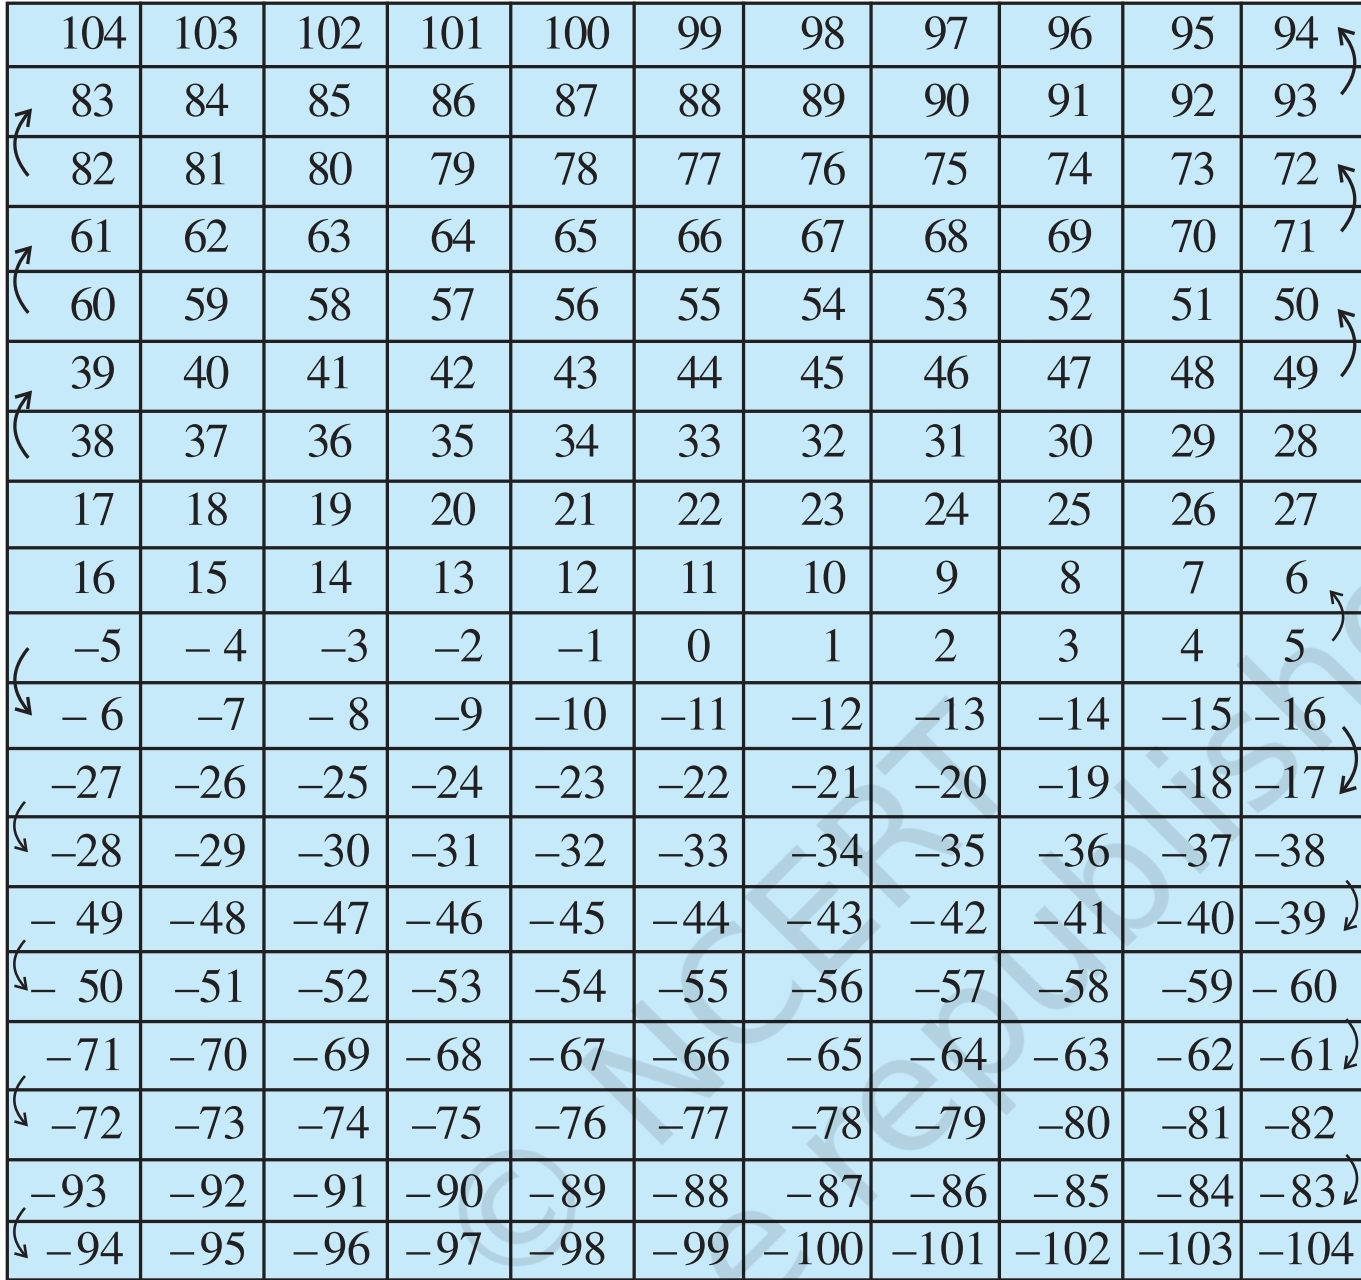
\includegraphics[width=\columnwidth]{figs/game1.jpg}
  \caption{}
  \label{fig:game1}
\end{figure}
\end{enumerate}
%
\begin{enumerate}[label=\thesection.\arabic*, ref=\thesection.\theenumi,resume*]
	\item Write a program to simulate the game.  Give the inputs manually.
	\\
	\solution 
	\lstinputlisting{codes/rv/game.c}
	\item Revise the program by generating the inputs randomly as follows 
		\begin{enumerate}
			\item Generate the numbers on all the dice using a uniform distribution ranging from 1 to 6.
			\item Simulate the blue and red dice through a Bernoulli distribution having values 1 and -1.
		\end{enumerate}
\end{enumerate}

\iffalse
\subsection{NCERT}
Verify
\begin{enumerate}[label=\thesubsection.\arabic*.,ref=\thesubsection.\theenumi,resume*]
	\item $x^3+y^3 = \brak{x+y}\brak{x^2-xy+y^2}$
	\item $x^3-y^3 = \brak{x-y}\brak{x^2+xy+y^2}$
	\item $x^3+y^3+z^3-3xyz = \frac{1}{2}\brak{x+y+z}\sbrak{\brak{x-y}^{2}+\brak{y-z}^{2}+\brak{z-x}^{2}}$
\end{enumerate}
Factorize each of the following
\begin{enumerate}[label=\thesubsection.\arabic*.,ref=\thesubsection.\theenumi]
	\item $8a^3+b^3+12a^2b+6ab^2$
	\item $8a^3-b^3-12a^2b+6ab^2$
	\item $27-125a^3-135a+225a^2$
	\item $64a^3-27b^3-144a^2b+108ab^2$
	\item $27p^3-\frac{1}{216}-\frac{9}{2}p^2 + \frac{p}{4}$
	\item $27y^3+125z^3$ 
	\item $64m^3-343n^3$
	\item $27x^3+y^3+z^3-9xyz$
\end{enumerate}
Find the value of each of the following 
\begin{enumerate}[label=\thesubsection.\arabic*.,ref=\thesubsection.\theenumi,resume*]
	\item $\brak{-12}^3+\brak{7}^3+\brak{5}^3$
	\item $\brak{28}^3+\brak{-15}^3+\brak{-13}^3$
\end{enumerate}
Give possible expressions for the length and breadth of each of the following rectangles, in which their areas are given
\begin{enumerate}[label=\thesubsection.\arabic*.,ref=\thesubsection.\theenumi,resume*]
	\item $25a^2-35a+12$
	\item $35a^2+13y-12$
\end{enumerate}
What are the possible expressions for the dimensions of the cuboids whose volumes are given below
\begin{enumerate}[label=\thesubsection.\arabic*.,ref=\thesubsection.\theenumi,resume*]
	\item $3x^2-12x$
	\item $12ky^2+8ky-20k$
\end{enumerate}

\section{Polynomials}
\subsection{NCERT}
\begin{enumerate}[label=\thesubsection.\arabic*, ref=\thesubsection.\theenumi,resume*]
%
\item Divide $p(x)$ by $g(x)$, where $p(x) = x + 3x^2– 1$ and $g(x) = 1 + x$.
\item Divide the polynomial $p(x) = 3x^4-4x^3-3x-1 $ by $x-1$.
\item Find the remainder obtained upon dividing $p(x) = x^3+1$ by $x+1$.
\item Find the remainder when $x^4+x^3-2x^2+x+1$ is divided by $x-1$.
\item Check whether the polynomial $q(t)=4t^3+4t^2-t-1$ is a multiple of $2t+1$.
\item Find the remainder when $x^3+3x^2+3x+1$ is divided by 
	\begin{enumerate}
		\item $x+1$
		\item $x-\frac{1}{2}$
		\item $x$
		\item $x+\pi$
		\item $5+2x$
	\end{enumerate}
\item Check whether $7+3x$ is a factor of $3x^3+7x$.
\item Find the value of $k$, if $x – 1$ is a factor of $p(x) = 4x^3+ 3x^2 - 4x + k$.
%
\item Determine which of the following polynomials has $x+1$ as a factor
	\begin{enumerate}
		\item $x^3+x^2+x+1$
		\item $x^4+x^3+x^2+x+1$
		\item $x^4+3x^3+3x^2+x+1$
		\item $x^3-x^2-\brak{2+\sqrt{2}}x+\sqrt{2}$
	\end{enumerate}
\item Factorize $x^3-23x^2+142x-120$.
\item Divide $2x^2+3x+1$ by $x+2$.
\item Divide $3x^3+x^2+2x+5$ by $1+2x+x^2$.
\item Find all the zeroes of $2x^4-3x^3-3x^2+6x-2$, if you know that two of its zeroes are $\sqrt{2}$ and $-\sqrt{2}$.
\item Find the remainder when $x^3-ax^2 +6x-a$ is divided by $x-a$.
\item Find the value of k, if x – 1 is a factor of p(x) in each of the following cases: 
\begin{enumerate}
\item $p(x) = x^2 + x + k$
\item $p(x) = kx^2-\sqrt{2}x+1$
\item $p(x) = 2x^2 + kx + \sqrt{2}$
\item $p(x) = kx^2  - 3x + k$
\end{enumerate}
\item Divide the polnyomial $p(x)$ by the polynomial $g(x)$ and find the quotient and remainder in each of the following:
\begin{enumerate}
\item $p(x) = x^3-3x^2+5x-3, g(x) = x^2-2$.
\item $p(x) = x^4-3x^2+4x+5, g(x) = x^2+1-x$.
\item $p(x) = x^4-5x+6, g(x) = 2-x^2$.
\end{enumerate}
\item Check whether the first polynomial is a factor of the second polynomial by dividing the second polynomial by the first polynomial:
\begin{enumerate}
\item $t^2-x,2t^4+3t^3-2t^2-9t-12$.
\item $x^2+3x+1, 3x^4+5x^3-7x^2+2x+2$.
\item $x^3-3x+1, x^5-4x^3+x^2+3x+1$.
\end{enumerate}
%
\item Obtain all the other zeroes of $3x^4+6x^3-2x^2-10x-5$, if two of its zeroes are $\sqrt{\frac{5}{3}}$and $-\sqrt{\frac{5}{3}}$.
\item On dividing $x^3-3x^2+x+2$ by a polynomial $g(x)$, the quotient and remainder were $x-2$ and $-2x+4$respectively.  Find $g(x)$.
\item Verify that the numbers given alongside the cubic polynomials below are their zeroes.  Also verify if the relationship between the zeroes and the coefficients in each case:
\begin{enumerate}
\item $2x^3+x^2-5x+2; \frac{1}{2}, 1, -2$
\item $x^3-4x^2+5x-2; 2, 1, 1$
\end{enumerate}
\item Find a cubic polynomial with the sum, sum of the product of its zeroes taken two at a time, and the product of its zeroes as 2, -7, -4 respectively.
\item If two zeroes of the polynomial $x^4-6x^3-26x^2+138x-35$ are $2\pm \sqrt{3}$, find the other zeroes.\item If the polynomial $x^4-6x^3+16x^2-25x+10$ is divided by another polynomial $x^2-2x+k$, the remainder comes out to be $x+a$, find $k$ and $a$.
\item Use the factor theorem to determine whether $g(x)$ is a factor of $p(x)$ in each of the following cases.
	\begin{enumerate}
		\item $p(x) = 2x^3+x^2-2x-1, g(x) = x+1$
		\item $p(x) = x^3+3x^2+3x+1, g(x) = x+2$
		\item $p(x) = x^3-4x^2+x+6, g(x) = x-3$
	\end{enumerate}
\item Factorise
	\begin{enumerate}
		\item $12x^2-7x + 1$
		\item $2x^2+7x + 3$
		\item $6x^2+5x - 6$
		\item $3x^2-x - 4$
		\item $x^3-2x^2 - x+2$
		\item $x^3-3x^2 - 9x-5$
		\item $x^3+13x^2 +32x+20$
		\item $2y^3+y^2 - 2y+1$
\end{enumerate}
\item Factorise $y^2-5y+6$ using the factor theorem.
\end{enumerate}

\section{Roots}
\subsection{NCERT}
Find the roots of the following equations graphically or otherwise.
\begin{enumerate}[label=\thesubsection.\arabic*, ref=\thesubsection.\theenumi]
	\begin{multicols}{2}
	\item $x^2-2x=0$
	\item $x^3-x^2+2=0$
	\item $x^5-x^4+3=0$
	\item $2-y^2-y^3+2y^8=0$
	\item $x-x^3=1$
	\item $5x^3+4x^2+7x=0$
	\item $4-y^2=0$
	\item $x^2+x+2 = 0$
	\item $4x^2-3x+7 = 0$
	\item $y^2+\sqrt{2} = 0$
	\item $3\sqrt{t}+t\sqrt{2} = 1$
	\item $y+\frac{2}{y} = 1$
	\item $x^2+x = 1$
	\item $y+{y}^2+4 = 0$
	\item $y(x)=5x^2-3x+7 = 0$.  Find $y(1).$
	\item $3y^3-4y+\sqrt{11}=0$.  Find $y(2).$
	\item $4t^4+5t^3-t^2+6=0$
	\item $5x^3-2x^2+3x-2=0$.  Find $y(1), y(0)$ and $y(-1)$.
	\item $5x-4x^2+3=0$.  Find $y(2), y(0)$ and $y(-1)$.
	\item $\brak{x-2}^2+1 = 2x-3$
	\item $x\brak{2x+3} = x^2+1$
	\item $\brak{x+2}^3 = x^3-4$
	\item $\brak{x+1}^2 = 2\brak{x-3}$
	\item $x^2-2x = -2\brak{3-x}$
	\item $\brak{2x-1}\brak{x-3} = \brak{x+5}\brak{x-1}$
	\item $\brak{x+2}^{3} = 2x\brak{x^2-1}$
	\item ${x}^{3}-4x^2-x+1 = \brak{x-2}^3$
	\item $2{x}^{2}-5x+3 = 0$
	\item $6{x}^{2}-x-2 = 0$
	\item $3{x}^{2}-2\sqrt{6}x+2 = 0$
	\item ${x}^{2}-3x-10 = 0$
	\item $2{x}^{2}+x-6 = 0$
	\item $\sqrt{2}{x}^{2}+7x+5\sqrt{2} = 0$
	\item $2{x}^{2}-x+\frac{1}{8} = 0$
	\item $100{x}^{2}-20x+1 = 0$
	\item $5{x}^{2}-6x-2 = 0$
	\item $4{x}^{2}+3x+5 = 0$
	\item $3{x}^{2}-5x+2 = 0$
	\item ${x}^{2}+4x+5 = 0$
	\item $2{x}^{2}-2\sqrt{2}x+1 = 0$
	\item $x+\frac{1}{x}=3, x\neq{0}$
\item $\frac{1}{x}-\frac{1}{x-2} = 3, x\neq 0,2$
\item $3x^2-2x+\frac{1}{3} = 0$. 
\item $x^2-4x+3 = 0$.
\item $2x^2-4x+3 = 0$.
\item $x-\frac{1}{x}=3, x\neq{0}$
\item
$\frac{1}{x+4}-\frac{1}{x-7}=\frac{11}{30}, x\neq{-4,7}$
\item $2x^2-3x+5=0$
\item $3x^2-4 \sqrt 3x+4=0$
\item $2x^2-6x+3=0$
	\end{multicols}
\end{enumerate}
Find $p(0), p(1)$ and $p(2)$ for each of the following polynomials.
\begin{enumerate}[label=\thesubsection.\arabic*, ref=\thesubsection.\theenumi,resume*]
	\begin{multicols}{2}
	\item $p(y)=y^2-y+1$
	\item $p(t)=2+t+2t^2-t^3$
	\item $p(x)=x^3$
	\item $p(x)=\brak{y-1}\brak{y+1}$
	\end{multicols}
\end{enumerate}
Find the values of $k$ for each of the following quadratic equations, so that they have two equal roots
\begin{enumerate}[label=\thesubsection.\arabic*, ref=\thesubsection.\theenumi,resume*]
\item 	$2x^2+kx+3 = 0$
\item 	$kx\brak{x-2}+6= 0$
\end{enumerate}
Verify whether the following are zeroes of the polynomial, indicated against them.
\begin{enumerate}[label=\thesubsection.\arabic*, ref=\thesubsection.\theenumi,resume*]
	\item $p(x) = x^2-1, \quad x=-1, 1$.
	\item $p(x) = \brak{x-2}\brak{x+1}, \quad x=-1, 2$.
	\item $p(x) = 3x^2-1, x=-\frac{1}{\sqrt{3}},\frac{2}{\sqrt{3}}$.
\end{enumerate}

\section{Quadratic Equations}
\subsection{NCERT}
\begin{enumerate}[label=\thesubsection.\arabic*,ref=\thesubsection.\theenumi]
%
	\item Janak and Jivanti together have 45 marbles. Both of them lost 5 marbles each, and the product of the number of marbles they now have is 124. We would like to find out how many marbles they had to start with.
\item  A cottage industry produces a certain number of toys in a day. The cost of production of each toy (in rupees) was found to be 55 minus the number of toys produced in a day. On a particular day, the total cost of production was \rupee 750. We would like to find out the number of toys produced on that day.
\item The product of Sunita’s age (in years) two years ago and her age four years from now is one more than twice her present age. What is her present age?
\item Find two consecutive odd positive integers, sum of whose squares is 290.
\item A motor boat whose speed is 18 km/h in still water takes 1 hour more to go 24 km upstream than to return downstream to the same spot. Find the speed of the stream.
%
\item The product of two consecutive positive integers is 306. We need to find the integers.
\item Rohan’s mother is 26 years older than him. The product of their ages (in years) 3 years from now will be 360. We would like to find Rohan’s present age.
\item A train travels a distance of 480 km at a uniform speed. If the speed had been 8 km/h less, then it would have taken 3 hours more to cover the same distance. We need to find the speed of the train.
\item Find two numbers whose sum is 27 and product is 182. 
\item  Find two consecutive positive integers, sum of whose squares is 365. 
\item  A cottage industry produces a certain number of pottery articles in a day. It was observed on a particular day that the cost of production of each article (in rupees) was 3 more than twice the number of articles produced on that day. If the total cost of production on that day was \rupee 90, find the number of articles produced and the cost of each article.
\item The sum of the reciprocals of Raman’s ages, (in years) 3 years ago and 5 years from now is $\frac{1}{3}$.  Find his present age.
\item In a class test, the sum of Shefali’s marks in Mathematics and English is 30. Had she got 2 marks more in Mathematics and 3 marks less in English, the product of their marks would have been 210. Find her marks in the two subjects.
\item The difference of squares of two numbers is 180. The square of the smaller number is 8 times the larger number. Find the two numbers.
\item A train travels 360 km at a uniform speed. If the speed had been 5 km/h more, it would have taken 1 hour less for the same journey. Find the speed of the train.
\item Two water taps together can fill a tank in 9$\frac{3}{ 8}$
hours. The tap of larger diameter takes 10
hours less than the smaller one to fill the tank separately. Find the time in which each tap can separately fill the tank.
\item An express train takes 1 hour less than a passenger train to travel 132 km between Mysore and Bangalore (without taking into consideration the time they stop at intermediate stations). If the average speed of the express train is 11km/h more than that of the passenger train, find the average speed of the two trains.
\item Sum of the areas of two squares is 468 $m^22$ find the sides of the two squares.
\item Is the following situation possible? If so, determine their present ages. The sum of the ages of two friends is 20 years. Four years ago, the product of their ages in years was 48.
%
\item The area of a rectangular plot is $528m^2$.  The length of the plot is one more than twice the breadth. We need to find the length and breadth of the plot. 
\item A temple courtyard has a carpet area of $300m^2$ with its length one metre more than twice its breadth.  What should be the length and breadth of the hall.
\item The altitude of a right triangle is $7cm$ less than its base. If the hypotenuse is $13 cm$, find the other two sides. 
\item A rectangular park is to be designed whose breadth is $3$ m less than its length. Its area is to be $4$ square metres than the area of a park that has already been made in the shape of a isoceles triangle with its base as  the breadth of the rectangular park and of altitude $12$ m. Find its length and breadth.
\item The diagonal of a rectangular field is $60$ metres more than the shorter side. If the longer side is $30$ metres more than the shorter side, find the sides of the field.
\item The difference of squares of two numbers is $180$. The square of the smaller number is $8$ times the larger number. Find the two numbers.
\item A train travels $360$ km at a uniform speed. If the speed had been $5$ km/hr more, it would have taken $1$ hour less for the same journey. Find the speed of the train.
\item Two water taps together can fill a tank in $9\frac{3}{8}$ hours. The tap of larger diameter takes $10$ hours. The tap of larger diameter takes $10$ hours less than the smaller one to fill the tank seperately. Find the time in which each tap can seperately fill the  tank.
\item A pole has to be erected at a point on the boundary of a circular park of diameter $1.3$ metres in such a way that the difference of its distances from two diametrically opposite fixed gates A and B on the boundary is $7$ metres. Is it possible to do so? If yes, at what distances from the two gatees should the pole be erected?
\item Sum of the areas of two squares is $468m^2$. If the difference of their perimeter is 24m, find the sides of the two squares.  
\item Is it possible to design a rectangular mango grove whose length is twice its breadth, and the area is  $800m^2$? If so, find its length and breadth.
\item Is the following situation possible? If so, determine their present ages.
\\ The sum of the ages of the two friends is 20 years. Four years ago, the product of their ages in years was $48$.
\item Is it possible to design a rectangular park of perimeter 80m and area of $400m^2$. If so, find its length and breadth.
\end{enumerate}

\subsection{Formulae}
\input{formulae/ap.tex}
\subsection{CBSE}
\input{cbse/ap.tex}
\subsection{JEE}
\input{jee/ap.tex}
\section{Geometric Progression}
\subsection{Formulae}
\input{formulae/gp.tex}
\subsection{NCERT}
\input{ncert/gp.tex}
\subsection{JEE}
\input{jee/gp.tex}
\section{$Z$ Transform}
\subsection{Formulae}
\input{formulae/zt.tex}
\subsection{NCERT}
\input{ncert/zt.tex}
\subsection{JEE}
\input{jee/zt.tex}
\section{Miscellaneous}
\subsection{NCERT}
\input{ncert/misc.tex}
\subsection{JEE}
\input{jee/misc.tex}
\section{Binomial Theorem}
\subsection{NCERT}
\input{ncert/binom.tex}
\subsection{JEE}
\input{jee/binom.tex}
%\input{jee/exp.tex}
\section{Others}
\subsection{JEE}
%\input{jee/other.tex}
\input{jee/exp.tex}
\subsection{CBSE}
\input{cbse/hd.tex}
\subsection{JEE}
\input{JEE/hd.tex}
%
\section{Triangle}
\subsection{NCERT}
%%%%%%%%%%%%%%%%%%%%%%%%%%%%%%%%%%%%%%%%%%%%%%%%%%%%%%%%%%%%%%%%%%%%%%
%%                                                                  %%
%%  This is the header of a LaTeX2e file exported from Gnumeric.    %%
%%                                                                  %%
%%  This file can be compiled as it stands or included in another   %%
%%  LaTeX document. The table is based on the longtable package so  %%
%%  the longtable options (headers, footers...) can be set in the   %%
%%  preamble section below (see PRAMBLE).                           %%
%%                                                                  %%
%%  To include the file in another, the following two lines must be %%
%%  in the including file:                                          %%
%%        \def\inputGnumericTable{}                                 %%
%%  at the beginning of the file and:                               %%
%%        \input{name-of-this-file.tex}                             %%
%%  where the table is to be placed. Note also that the including   %%
%%  file must use the following packages for the table to be        %%
%%  rendered correctly:                                             %%
%%    \usepackage[latin1]{inputenc}                                 %%
%%    \usepackage{color}                                            %%
%%    \usepackage{array}                                            %%
%%    \usepackage{longtable}                                        %%
%%    \usepackage{calc}                                             %%
%%    \usepackage{multirow}                                         %%
%%    \usepackage{hhline}                                           %%
%%    \usepackage{ifthen}                                           %%
%%  optionally (for landscape tables embedded in another document): %%
%%    \usepackage{lscape}                                           %%
%%                                                                  %%
%%%%%%%%%%%%%%%%%%%%%%%%%%%%%%%%%%%%%%%%%%%%%%%%%%%%%%%%%%%%%%%%%%%%%%



%%  This section checks if we are begin input into another file or  %%
%%  the file will be compiled alone. First use a macro taken from   %%
%%  the TeXbook ex 7.7 (suggestion of Han-Wen Nienhuys).            %%
\def\ifundefined#1{\expandafter\ifx\csname#1\endcsname\relax}


%%  Check for the \def token for inputed files. If it is not        %%
%%  defined, the file will be processed as a standalone and the     %%
%%  preamble will be used.                                          %%
\ifundefined{inputGnumericTable}

%%  We must be able to close or not the document at the end.        %%
	\def\gnumericTableEnd{\end{document}}


%%%%%%%%%%%%%%%%%%%%%%%%%%%%%%%%%%%%%%%%%%%%%%%%%%%%%%%%%%%%%%%%%%%%%%
%%                                                                  %%
%%  This is the PREAMBLE. Change these values to get the right      %%
%%  paper size and other niceties.                                  %%
%%                                                                  %%
%%%%%%%%%%%%%%%%%%%%%%%%%%%%%%%%%%%%%%%%%%%%%%%%%%%%%%%%%%%%%%%%%%%%%%

	\documentclass[12pt%
			  ,landscape%
                    ]{report}
       \usepackage[latin1]{inputenc}
       \usepackage{fullpage}
       \usepackage{color}
       \usepackage{array}
       \usepackage{longtable}
       \usepackage{calc}
       \usepackage{multirow}
       \usepackage{hhline}
       \usepackage{ifthen}

	\begin{document}


%%  End of the preamble for the standalone. The next section is for %%
%%  documents which are included into other LaTeX2e files.          %%
\else

%%  We are not a stand alone document. For a regular table, we will %%
%%  have no preamble and only define the closing to mean nothing.   %%
    \def\gnumericTableEnd{}

%%  If we want landscape mode in an embedded document, comment out  %%
%%  the line above and uncomment the two below. The table will      %%
%%  begin on a new page and run in landscape mode.                  %%
%       \def\gnumericTableEnd{\end{landscape}}
%       \begin{landscape}


%%  End of the else clause for this file being \input.              %%
\fi

%%%%%%%%%%%%%%%%%%%%%%%%%%%%%%%%%%%%%%%%%%%%%%%%%%%%%%%%%%%%%%%%%%%%%%
%%                                                                  %%
%%  The rest is the gnumeric table, except for the closing          %%
%%  statement. Changes below will alter the table's appearance.     %%
%%                                                                  %%
%%%%%%%%%%%%%%%%%%%%%%%%%%%%%%%%%%%%%%%%%%%%%%%%%%%%%%%%%%%%%%%%%%%%%%

\providecommand{\gnumericmathit}[1]{#1} 
%%  Uncomment the next line if you would like your numbers to be in %%
%%  italics if they are italizised in the gnumeric table.           %%
%\renewcommand{\gnumericmathit}[1]{\mathit{#1}}
\providecommand{\gnumericPB}[1]%
{\let\gnumericTemp=\\#1\let\\=\gnumericTemp\hspace{0pt}}
 \ifundefined{gnumericTableWidthDefined}
        \newlength{\gnumericTableWidth}
        \newlength{\gnumericTableWidthComplete}
        \newlength{\gnumericMultiRowLength}
        \global\def\gnumericTableWidthDefined{}
 \fi
%% The following setting protects this code from babel shorthands.  %%
 \ifthenelse{\isundefined{\languageshorthands}}{}{\languageshorthands{english}}
%%  The default table format retains the relative column widths of  %%
%%  gnumeric. They can easily be changed to c, r or l. In that case %%
%%  you may want to comment out the next line and uncomment the one %%
%%  thereafter                                                      %%
\providecommand\gnumbox{\makebox[0pt]}
%%\providecommand\gnumbox[1][]{\makebox}

%% to adjust positions in multirow situations                       %%
\setlength{\bigstrutjot}{\jot}
\setlength{\extrarowheight}{\doublerulesep}

%%  The \setlongtables command keeps column widths the same across  %%
%%  pages. Simply comment out next line for varying column widths.  %%
\setlongtables

\setlength\gnumericTableWidth{%
	41pt+%
	45pt+%
	125pt+%
0pt}
\def\gumericNumCols{3}
\setlength\gnumericTableWidthComplete{\gnumericTableWidth+%
         \tabcolsep*\gumericNumCols*2+\arrayrulewidth*\gumericNumCols}
\ifthenelse{\lengthtest{\gnumericTableWidthComplete > \linewidth}}%
         {\def\gnumericScale{1*\ratio{\linewidth-%
                        \tabcolsep*\gumericNumCols*2-%
                        \arrayrulewidth*\gumericNumCols}%
{\gnumericTableWidth}}}%
{\def\gnumericScale{1}}

%%%%%%%%%%%%%%%%%%%%%%%%%%%%%%%%%%%%%%%%%%%%%%%%%%%%%%%%%%%%%%%%%%%%%%
%%                                                                  %%
%% The following are the widths of the various columns. We are      %%
%% defining them here because then they are easier to change.       %%
%% Depending on the cell formats we may use them more than once.    %%
%%                                                                  %%
%%%%%%%%%%%%%%%%%%%%%%%%%%%%%%%%%%%%%%%%%%%%%%%%%%%%%%%%%%%%%%%%%%%%%%

\ifthenelse{\isundefined{\gnumericColA}}{\newlength{\gnumericColA}}{}\settowidth{\gnumericColA}{\begin{tabular}{@{}p{41pt*\gnumericScale}@{}}x\end{tabular}}
\ifthenelse{\isundefined{\gnumericColB}}{\newlength{\gnumericColB}}{}\settowidth{\gnumericColB}{\begin{tabular}{@{}p{45pt*\gnumericScale}@{}}x\end{tabular}}
\ifthenelse{\isundefined{\gnumericColC}}{\newlength{\gnumericColC}}{}\settowidth{\gnumericColC}{\begin{tabular}{@{}p{125pt*\gnumericScale}@{}}x\end{tabular}}

\begin{longtable}[c]{%
	b{\gnumericColA}%
	b{\gnumericColB}%
	b{\gnumericColC}%
	}

%%%%%%%%%%%%%%%%%%%%%%%%%%%%%%%%%%%%%%%%%%%%%%%%%%%%%%%%%%%%%%%%%%%%%%
%%  The longtable options. (Caption, headers... see Goosens, p.124) %%
%	\caption{The Table Caption.}             \\	%
% \hline	% Across the top of the table.
%%  The rest of these options are table rows which are placed on    %%
%%  the first, last or every page. Use \multicolumn if you want.    %%

%%  Header for the first page.                                      %%
%	\multicolumn{3}{c}{The First Header} \\ \hline 
%	\multicolumn{1}{c}{colTag}	%Column 1
%	&\multicolumn{1}{c}{colTag}	%Column 2
%	&\multicolumn{1}{c}{colTag}	\\ \hline %Last column
%	\endfirsthead

%%  The running header definition.                                  %%
%	\hline
%	\multicolumn{3}{l}{\ldots\small\slshape continued} \\ \hline
%	\multicolumn{1}{c}{colTag}	%Column 1
%	&\multicolumn{1}{c}{colTag}	%Column 2
%	&\multicolumn{1}{c}{colTag}	\\ \hline %Last column
%	\endhead

%%  The running footer definition.                                  %%
%	\hline
%	\multicolumn{3}{r}{\small\slshape continued\ldots} \\
%	\endfoot

%%  The ending footer definition.                                   %%
%	\multicolumn{3}{c}{That's all folks} \\ \hline 
%	\endlastfoot
%%%%%%%%%%%%%%%%%%%%%%%%%%%%%%%%%%%%%%%%%%%%%%%%%%%%%%%%%%%%%%%%%%%%%%

\hhline{|-|-|-}
	 \multicolumn{1}{|p{\gnumericColA}|}%
	{\gnumericPB{\centering}\textbf{Base}}
	&\multicolumn{1}{p{\gnumericColB}|}%
	{\gnumericPB{\centering}\textbf{Height}}
	&\multicolumn{1}{p{\gnumericColC}|}%
	{\gnumericPB{\centering}\textbf{Area of Triangle}}
\\
\hhline{|---|}
	 \multicolumn{1}{|p{\gnumericColA}|}%
	{\gnumericPB{\centering}15$cm$}
	&\multicolumn{1}{p{\gnumericColB}|}%
	{}
	&\multicolumn{1}{p{\gnumericColC}|}%
	{\gnumericPB{\centering}87$cm^2$}
\\
\hhline{|---|}
	 \multicolumn{1}{|p{\gnumericColA}|}%
	{}
	&\multicolumn{1}{p{\gnumericColB}|}%
	{\gnumericPB{\centering}\gnumbox{31.4$mm$}}
	&\multicolumn{1}{p{\gnumericColC}|}%
	{\gnumericPB{\centering}\gnumbox{1256$mm^2$}}
\\
\hhline{|---|}
	 \multicolumn{1}{|p{\gnumericColA}|}%
	{\gnumericPB{\centering}\gnumbox{22$cm$}}
	&\multicolumn{1}{p{\gnumericColB}|}%
	{}
	&\multicolumn{1}{p{\gnumericColC}|}%
	{\gnumericPB{\centering}\gnumbox{170.5$cm^2$}}
\\
\hhline{|-|-|-|}
\end{longtable}

\ifthenelse{\isundefined{\languageshorthands}}{}{\languageshorthands{\languagename}}
\gnumericTableEnd

\subsection{CBSE}
%%%%%%%%%%%%%%%%%%%%%%%%%%%%%%%%%%%%%%%%%%%%%%%%%%%%%%%%%%%%%%%%%%%%%%
%%                                                                  %%
%%  This is the header of a LaTeX2e file exported from Gnumeric.    %%
%%                                                                  %%
%%  This file can be compiled as it stands or included in another   %%
%%  LaTeX document. The table is based on the longtable package so  %%
%%  the longtable options (headers, footers...) can be set in the   %%
%%  preamble section below (see PRAMBLE).                           %%
%%                                                                  %%
%%  To include the file in another, the following two lines must be %%
%%  in the including file:                                          %%
%%        \def\inputGnumericTable{}                                 %%
%%  at the beginning of the file and:                               %%
%%        \input{name-of-this-file.tex}                             %%
%%  where the table is to be placed. Note also that the including   %%
%%  file must use the following packages for the table to be        %%
%%  rendered correctly:                                             %%
%%    \usepackage[latin1]{inputenc}                                 %%
%%    \usepackage{color}                                            %%
%%    \usepackage{array}                                            %%
%%    \usepackage{longtable}                                        %%
%%    \usepackage{calc}                                             %%
%%    \usepackage{multirow}                                         %%
%%    \usepackage{hhline}                                           %%
%%    \usepackage{ifthen}                                           %%
%%  optionally (for landscape tables embedded in another document): %%
%%    \usepackage{lscape}                                           %%
%%                                                                  %%
%%%%%%%%%%%%%%%%%%%%%%%%%%%%%%%%%%%%%%%%%%%%%%%%%%%%%%%%%%%%%%%%%%%%%%



%%  This section checks if we are begin input into another file or  %%
%%  the file will be compiled alone. First use a macro taken from   %%
%%  the TeXbook ex 7.7 (suggestion of Han-Wen Nienhuys).            %%
\def\ifundefined#1{\expandafter\ifx\csname#1\endcsname\relax}


%%  Check for the \def token for inputed files. If it is not        %%
%%  defined, the file will be processed as a standalone and the     %%
%%  preamble will be used.                                          %%
\ifundefined{inputGnumericTable}

%%  We must be able to close or not the document at the end.        %%
	\def\gnumericTableEnd{\end{document}}


%%%%%%%%%%%%%%%%%%%%%%%%%%%%%%%%%%%%%%%%%%%%%%%%%%%%%%%%%%%%%%%%%%%%%%
%%                                                                  %%
%%  This is the PREAMBLE. Change these values to get the right      %%
%%  paper size and other niceties.                                  %%
%%                                                                  %%
%%%%%%%%%%%%%%%%%%%%%%%%%%%%%%%%%%%%%%%%%%%%%%%%%%%%%%%%%%%%%%%%%%%%%%

	\documentclass[12pt%
			  ,landscape%
                    ]{report}
       \usepackage[latin1]{inputenc}
       \usepackage{fullpage}
       \usepackage{color}
       \usepackage{array}
       \usepackage{longtable}
       \usepackage{calc}
       \usepackage{multirow}
       \usepackage{hhline}
       \usepackage{ifthen}

	\begin{document}


%%  End of the preamble for the standalone. The next section is for %%
%%  documents which are included into other LaTeX2e files.          %%
\else

%%  We are not a stand alone document. For a regular table, we will %%
%%  have no preamble and only define the closing to mean nothing.   %%
    \def\gnumericTableEnd{}

%%  If we want landscape mode in an embedded document, comment out  %%
%%  the line above and uncomment the two below. The table will      %%
%%  begin on a new page and run in landscape mode.                  %%
%       \def\gnumericTableEnd{\end{landscape}}
%       \begin{landscape}


%%  End of the else clause for this file being \input.              %%
\fi

%%%%%%%%%%%%%%%%%%%%%%%%%%%%%%%%%%%%%%%%%%%%%%%%%%%%%%%%%%%%%%%%%%%%%%
%%                                                                  %%
%%  The rest is the gnumeric table, except for the closing          %%
%%  statement. Changes below will alter the table's appearance.     %%
%%                                                                  %%
%%%%%%%%%%%%%%%%%%%%%%%%%%%%%%%%%%%%%%%%%%%%%%%%%%%%%%%%%%%%%%%%%%%%%%

\providecommand{\gnumericmathit}[1]{#1} 
%%  Uncomment the next line if you would like your numbers to be in %%
%%  italics if they are italizised in the gnumeric table.           %%
%\renewcommand{\gnumericmathit}[1]{\mathit{#1}}
\providecommand{\gnumericPB}[1]%
{\let\gnumericTemp=\\#1\let\\=\gnumericTemp\hspace{0pt}}
 \ifundefined{gnumericTableWidthDefined}
        \newlength{\gnumericTableWidth}
        \newlength{\gnumericTableWidthComplete}
        \newlength{\gnumericMultiRowLength}
        \global\def\gnumericTableWidthDefined{}
 \fi
%% The following setting protects this code from babel shorthands.  %%
 \ifthenelse{\isundefined{\languageshorthands}}{}{\languageshorthands{english}}
%%  The default table format retains the relative column widths of  %%
%%  gnumeric. They can easily be changed to c, r or l. In that case %%
%%  you may want to comment out the next line and uncomment the one %%
%%  thereafter                                                      %%
\providecommand\gnumbox{\makebox[0pt]}
%%\providecommand\gnumbox[1][]{\makebox}

%% to adjust positions in multirow situations                       %%
\setlength{\bigstrutjot}{\jot}
\setlength{\extrarowheight}{\doublerulesep}

%%  The \setlongtables command keeps column widths the same across  %%
%%  pages. Simply comment out next line for varying column widths.  %%
\setlongtables

\setlength\gnumericTableWidth{%
	41pt+%
	45pt+%
	125pt+%
0pt}
\def\gumericNumCols{3}
\setlength\gnumericTableWidthComplete{\gnumericTableWidth+%
         \tabcolsep*\gumericNumCols*2+\arrayrulewidth*\gumericNumCols}
\ifthenelse{\lengthtest{\gnumericTableWidthComplete > \linewidth}}%
         {\def\gnumericScale{1*\ratio{\linewidth-%
                        \tabcolsep*\gumericNumCols*2-%
                        \arrayrulewidth*\gumericNumCols}%
{\gnumericTableWidth}}}%
{\def\gnumericScale{1}}

%%%%%%%%%%%%%%%%%%%%%%%%%%%%%%%%%%%%%%%%%%%%%%%%%%%%%%%%%%%%%%%%%%%%%%
%%                                                                  %%
%% The following are the widths of the various columns. We are      %%
%% defining them here because then they are easier to change.       %%
%% Depending on the cell formats we may use them more than once.    %%
%%                                                                  %%
%%%%%%%%%%%%%%%%%%%%%%%%%%%%%%%%%%%%%%%%%%%%%%%%%%%%%%%%%%%%%%%%%%%%%%

\ifthenelse{\isundefined{\gnumericColA}}{\newlength{\gnumericColA}}{}\settowidth{\gnumericColA}{\begin{tabular}{@{}p{41pt*\gnumericScale}@{}}x\end{tabular}}
\ifthenelse{\isundefined{\gnumericColB}}{\newlength{\gnumericColB}}{}\settowidth{\gnumericColB}{\begin{tabular}{@{}p{45pt*\gnumericScale}@{}}x\end{tabular}}
\ifthenelse{\isundefined{\gnumericColC}}{\newlength{\gnumericColC}}{}\settowidth{\gnumericColC}{\begin{tabular}{@{}p{125pt*\gnumericScale}@{}}x\end{tabular}}

\begin{longtable}[c]{%
	b{\gnumericColA}%
	b{\gnumericColB}%
	b{\gnumericColC}%
	}

%%%%%%%%%%%%%%%%%%%%%%%%%%%%%%%%%%%%%%%%%%%%%%%%%%%%%%%%%%%%%%%%%%%%%%
%%  The longtable options. (Caption, headers... see Goosens, p.124) %%
%	\caption{The Table Caption.}             \\	%
% \hline	% Across the top of the table.
%%  The rest of these options are table rows which are placed on    %%
%%  the first, last or every page. Use \multicolumn if you want.    %%

%%  Header for the first page.                                      %%
%	\multicolumn{3}{c}{The First Header} \\ \hline 
%	\multicolumn{1}{c}{colTag}	%Column 1
%	&\multicolumn{1}{c}{colTag}	%Column 2
%	&\multicolumn{1}{c}{colTag}	\\ \hline %Last column
%	\endfirsthead

%%  The running header definition.                                  %%
%	\hline
%	\multicolumn{3}{l}{\ldots\small\slshape continued} \\ \hline
%	\multicolumn{1}{c}{colTag}	%Column 1
%	&\multicolumn{1}{c}{colTag}	%Column 2
%	&\multicolumn{1}{c}{colTag}	\\ \hline %Last column
%	\endhead

%%  The running footer definition.                                  %%
%	\hline
%	\multicolumn{3}{r}{\small\slshape continued\ldots} \\
%	\endfoot

%%  The ending footer definition.                                   %%
%	\multicolumn{3}{c}{That's all folks} \\ \hline 
%	\endlastfoot
%%%%%%%%%%%%%%%%%%%%%%%%%%%%%%%%%%%%%%%%%%%%%%%%%%%%%%%%%%%%%%%%%%%%%%

\hhline{|-|-|-}
	 \multicolumn{1}{|p{\gnumericColA}|}%
	{\gnumericPB{\centering}\textbf{Base}}
	&\multicolumn{1}{p{\gnumericColB}|}%
	{\gnumericPB{\centering}\textbf{Height}}
	&\multicolumn{1}{p{\gnumericColC}|}%
	{\gnumericPB{\centering}\textbf{Area of Triangle}}
\\
\hhline{|---|}
	 \multicolumn{1}{|p{\gnumericColA}|}%
	{\gnumericPB{\centering}15$cm$}
	&\multicolumn{1}{p{\gnumericColB}|}%
	{}
	&\multicolumn{1}{p{\gnumericColC}|}%
	{\gnumericPB{\centering}87$cm^2$}
\\
\hhline{|---|}
	 \multicolumn{1}{|p{\gnumericColA}|}%
	{}
	&\multicolumn{1}{p{\gnumericColB}|}%
	{\gnumericPB{\centering}\gnumbox{31.4$mm$}}
	&\multicolumn{1}{p{\gnumericColC}|}%
	{\gnumericPB{\centering}\gnumbox{1256$mm^2$}}
\\
\hhline{|---|}
	 \multicolumn{1}{|p{\gnumericColA}|}%
	{\gnumericPB{\centering}\gnumbox{22$cm$}}
	&\multicolumn{1}{p{\gnumericColB}|}%
	{}
	&\multicolumn{1}{p{\gnumericColC}|}%
	{\gnumericPB{\centering}\gnumbox{170.5$cm^2$}}
\\
\hhline{|-|-|-|}
\end{longtable}

\ifthenelse{\isundefined{\languageshorthands}}{}{\languageshorthands{\languagename}}
\gnumericTableEnd

\subsection{JEE}
 %%%%%%%%%%%%%%%%%%%%%%%%%%%%%%%%%%%%%%%%%%%%%%%%%%%%%%%%%%%%%%%%%%%%%%
%%                                                                  %%
%%  This is the header of a LaTeX2e file exported from Gnumeric.    %%
%%                                                                  %%
%%  This file can be compiled as it stands or included in another   %%
%%  LaTeX document. The table is based on the longtable package so  %%
%%  the longtable options (headers, footers...) can be set in the   %%
%%  preamble section below (see PRAMBLE).                           %%
%%                                                                  %%
%%  To include the file in another, the following two lines must be %%
%%  in the including file:                                          %%
%%        \def\inputGnumericTable{}                                 %%
%%  at the beginning of the file and:                               %%
%%        \input{name-of-this-file.tex}                             %%
%%  where the table is to be placed. Note also that the including   %%
%%  file must use the following packages for the table to be        %%
%%  rendered correctly:                                             %%
%%    \usepackage[latin1]{inputenc}                                 %%
%%    \usepackage{color}                                            %%
%%    \usepackage{array}                                            %%
%%    \usepackage{longtable}                                        %%
%%    \usepackage{calc}                                             %%
%%    \usepackage{multirow}                                         %%
%%    \usepackage{hhline}                                           %%
%%    \usepackage{ifthen}                                           %%
%%  optionally (for landscape tables embedded in another document): %%
%%    \usepackage{lscape}                                           %%
%%                                                                  %%
%%%%%%%%%%%%%%%%%%%%%%%%%%%%%%%%%%%%%%%%%%%%%%%%%%%%%%%%%%%%%%%%%%%%%%



%%  This section checks if we are begin input into another file or  %%
%%  the file will be compiled alone. First use a macro taken from   %%
%%  the TeXbook ex 7.7 (suggestion of Han-Wen Nienhuys).            %%
\def\ifundefined#1{\expandafter\ifx\csname#1\endcsname\relax}


%%  Check for the \def token for inputed files. If it is not        %%
%%  defined, the file will be processed as a standalone and the     %%
%%  preamble will be used.                                          %%
\ifundefined{inputGnumericTable}

%%  We must be able to close or not the document at the end.        %%
	\def\gnumericTableEnd{\end{document}}


%%%%%%%%%%%%%%%%%%%%%%%%%%%%%%%%%%%%%%%%%%%%%%%%%%%%%%%%%%%%%%%%%%%%%%
%%                                                                  %%
%%  This is the PREAMBLE. Change these values to get the right      %%
%%  paper size and other niceties.                                  %%
%%                                                                  %%
%%%%%%%%%%%%%%%%%%%%%%%%%%%%%%%%%%%%%%%%%%%%%%%%%%%%%%%%%%%%%%%%%%%%%%

	\documentclass[12pt%
			  ,landscape%
                    ]{report}
       \usepackage[latin1]{inputenc}
       \usepackage{fullpage}
       \usepackage{color}
       \usepackage{array}
       \usepackage{longtable}
       \usepackage{calc}
       \usepackage{multirow}
       \usepackage{hhline}
       \usepackage{ifthen}

	\begin{document}


%%  End of the preamble for the standalone. The next section is for %%
%%  documents which are included into other LaTeX2e files.          %%
\else

%%  We are not a stand alone document. For a regular table, we will %%
%%  have no preamble and only define the closing to mean nothing.   %%
    \def\gnumericTableEnd{}

%%  If we want landscape mode in an embedded document, comment out  %%
%%  the line above and uncomment the two below. The table will      %%
%%  begin on a new page and run in landscape mode.                  %%
%       \def\gnumericTableEnd{\end{landscape}}
%       \begin{landscape}


%%  End of the else clause for this file being \input.              %%
\fi

%%%%%%%%%%%%%%%%%%%%%%%%%%%%%%%%%%%%%%%%%%%%%%%%%%%%%%%%%%%%%%%%%%%%%%
%%                                                                  %%
%%  The rest is the gnumeric table, except for the closing          %%
%%  statement. Changes below will alter the table's appearance.     %%
%%                                                                  %%
%%%%%%%%%%%%%%%%%%%%%%%%%%%%%%%%%%%%%%%%%%%%%%%%%%%%%%%%%%%%%%%%%%%%%%

\providecommand{\gnumericmathit}[1]{#1} 
%%  Uncomment the next line if you would like your numbers to be in %%
%%  italics if they are italizised in the gnumeric table.           %%
%\renewcommand{\gnumericmathit}[1]{\mathit{#1}}
\providecommand{\gnumericPB}[1]%
{\let\gnumericTemp=\\#1\let\\=\gnumericTemp\hspace{0pt}}
 \ifundefined{gnumericTableWidthDefined}
        \newlength{\gnumericTableWidth}
        \newlength{\gnumericTableWidthComplete}
        \newlength{\gnumericMultiRowLength}
        \global\def\gnumericTableWidthDefined{}
 \fi
%% The following setting protects this code from babel shorthands.  %%
 \ifthenelse{\isundefined{\languageshorthands}}{}{\languageshorthands{english}}
%%  The default table format retains the relative column widths of  %%
%%  gnumeric. They can easily be changed to c, r or l. In that case %%
%%  you may want to comment out the next line and uncomment the one %%
%%  thereafter                                                      %%
\providecommand\gnumbox{\makebox[0pt]}
%%\providecommand\gnumbox[1][]{\makebox}

%% to adjust positions in multirow situations                       %%
\setlength{\bigstrutjot}{\jot}
\setlength{\extrarowheight}{\doublerulesep}

%%  The \setlongtables command keeps column widths the same across  %%
%%  pages. Simply comment out next line for varying column widths.  %%
\setlongtables

\setlength\gnumericTableWidth{%
	41pt+%
	45pt+%
	125pt+%
0pt}
\def\gumericNumCols{3}
\setlength\gnumericTableWidthComplete{\gnumericTableWidth+%
         \tabcolsep*\gumericNumCols*2+\arrayrulewidth*\gumericNumCols}
\ifthenelse{\lengthtest{\gnumericTableWidthComplete > \linewidth}}%
         {\def\gnumericScale{1*\ratio{\linewidth-%
                        \tabcolsep*\gumericNumCols*2-%
                        \arrayrulewidth*\gumericNumCols}%
{\gnumericTableWidth}}}%
{\def\gnumericScale{1}}

%%%%%%%%%%%%%%%%%%%%%%%%%%%%%%%%%%%%%%%%%%%%%%%%%%%%%%%%%%%%%%%%%%%%%%
%%                                                                  %%
%% The following are the widths of the various columns. We are      %%
%% defining them here because then they are easier to change.       %%
%% Depending on the cell formats we may use them more than once.    %%
%%                                                                  %%
%%%%%%%%%%%%%%%%%%%%%%%%%%%%%%%%%%%%%%%%%%%%%%%%%%%%%%%%%%%%%%%%%%%%%%

\ifthenelse{\isundefined{\gnumericColA}}{\newlength{\gnumericColA}}{}\settowidth{\gnumericColA}{\begin{tabular}{@{}p{41pt*\gnumericScale}@{}}x\end{tabular}}
\ifthenelse{\isundefined{\gnumericColB}}{\newlength{\gnumericColB}}{}\settowidth{\gnumericColB}{\begin{tabular}{@{}p{45pt*\gnumericScale}@{}}x\end{tabular}}
\ifthenelse{\isundefined{\gnumericColC}}{\newlength{\gnumericColC}}{}\settowidth{\gnumericColC}{\begin{tabular}{@{}p{125pt*\gnumericScale}@{}}x\end{tabular}}

\begin{longtable}[c]{%
	b{\gnumericColA}%
	b{\gnumericColB}%
	b{\gnumericColC}%
	}

%%%%%%%%%%%%%%%%%%%%%%%%%%%%%%%%%%%%%%%%%%%%%%%%%%%%%%%%%%%%%%%%%%%%%%
%%  The longtable options. (Caption, headers... see Goosens, p.124) %%
%	\caption{The Table Caption.}             \\	%
% \hline	% Across the top of the table.
%%  The rest of these options are table rows which are placed on    %%
%%  the first, last or every page. Use \multicolumn if you want.    %%

%%  Header for the first page.                                      %%
%	\multicolumn{3}{c}{The First Header} \\ \hline 
%	\multicolumn{1}{c}{colTag}	%Column 1
%	&\multicolumn{1}{c}{colTag}	%Column 2
%	&\multicolumn{1}{c}{colTag}	\\ \hline %Last column
%	\endfirsthead

%%  The running header definition.                                  %%
%	\hline
%	\multicolumn{3}{l}{\ldots\small\slshape continued} \\ \hline
%	\multicolumn{1}{c}{colTag}	%Column 1
%	&\multicolumn{1}{c}{colTag}	%Column 2
%	&\multicolumn{1}{c}{colTag}	\\ \hline %Last column
%	\endhead

%%  The running footer definition.                                  %%
%	\hline
%	\multicolumn{3}{r}{\small\slshape continued\ldots} \\
%	\endfoot

%%  The ending footer definition.                                   %%
%	\multicolumn{3}{c}{That's all folks} \\ \hline 
%	\endlastfoot
%%%%%%%%%%%%%%%%%%%%%%%%%%%%%%%%%%%%%%%%%%%%%%%%%%%%%%%%%%%%%%%%%%%%%%

\hhline{|-|-|-}
	 \multicolumn{1}{|p{\gnumericColA}|}%
	{\gnumericPB{\centering}\textbf{Base}}
	&\multicolumn{1}{p{\gnumericColB}|}%
	{\gnumericPB{\centering}\textbf{Height}}
	&\multicolumn{1}{p{\gnumericColC}|}%
	{\gnumericPB{\centering}\textbf{Area of Triangle}}
\\
\hhline{|---|}
	 \multicolumn{1}{|p{\gnumericColA}|}%
	{\gnumericPB{\centering}15$cm$}
	&\multicolumn{1}{p{\gnumericColB}|}%
	{}
	&\multicolumn{1}{p{\gnumericColC}|}%
	{\gnumericPB{\centering}87$cm^2$}
\\
\hhline{|---|}
	 \multicolumn{1}{|p{\gnumericColA}|}%
	{}
	&\multicolumn{1}{p{\gnumericColB}|}%
	{\gnumericPB{\centering}\gnumbox{31.4$mm$}}
	&\multicolumn{1}{p{\gnumericColC}|}%
	{\gnumericPB{\centering}\gnumbox{1256$mm^2$}}
\\
\hhline{|---|}
	 \multicolumn{1}{|p{\gnumericColA}|}%
	{\gnumericPB{\centering}\gnumbox{22$cm$}}
	&\multicolumn{1}{p{\gnumericColB}|}%
	{}
	&\multicolumn{1}{p{\gnumericColC}|}%
	{\gnumericPB{\centering}\gnumbox{170.5$cm^2$}}
\\
\hhline{|-|-|-|}
\end{longtable}

\ifthenelse{\isundefined{\languageshorthands}}{}{\languageshorthands{\languagename}}
\gnumericTableEnd

\subsection{Olympiad}
%%%%%%%%%%%%%%%%%%%%%%%%%%%%%%%%%%%%%%%%%%%%%%%%%%%%%%%%%%%%%%%%%%%%%%
%%                                                                  %%
%%  This is the header of a LaTeX2e file exported from Gnumeric.    %%
%%                                                                  %%
%%  This file can be compiled as it stands or included in another   %%
%%  LaTeX document. The table is based on the longtable package so  %%
%%  the longtable options (headers, footers...) can be set in the   %%
%%  preamble section below (see PRAMBLE).                           %%
%%                                                                  %%
%%  To include the file in another, the following two lines must be %%
%%  in the including file:                                          %%
%%        \def\inputGnumericTable{}                                 %%
%%  at the beginning of the file and:                               %%
%%        \input{name-of-this-file.tex}                             %%
%%  where the table is to be placed. Note also that the including   %%
%%  file must use the following packages for the table to be        %%
%%  rendered correctly:                                             %%
%%    \usepackage[latin1]{inputenc}                                 %%
%%    \usepackage{color}                                            %%
%%    \usepackage{array}                                            %%
%%    \usepackage{longtable}                                        %%
%%    \usepackage{calc}                                             %%
%%    \usepackage{multirow}                                         %%
%%    \usepackage{hhline}                                           %%
%%    \usepackage{ifthen}                                           %%
%%  optionally (for landscape tables embedded in another document): %%
%%    \usepackage{lscape}                                           %%
%%                                                                  %%
%%%%%%%%%%%%%%%%%%%%%%%%%%%%%%%%%%%%%%%%%%%%%%%%%%%%%%%%%%%%%%%%%%%%%%



%%  This section checks if we are begin input into another file or  %%
%%  the file will be compiled alone. First use a macro taken from   %%
%%  the TeXbook ex 7.7 (suggestion of Han-Wen Nienhuys).            %%
\def\ifundefined#1{\expandafter\ifx\csname#1\endcsname\relax}


%%  Check for the \def token for inputed files. If it is not        %%
%%  defined, the file will be processed as a standalone and the     %%
%%  preamble will be used.                                          %%
\ifundefined{inputGnumericTable}

%%  We must be able to close or not the document at the end.        %%
	\def\gnumericTableEnd{\end{document}}


%%%%%%%%%%%%%%%%%%%%%%%%%%%%%%%%%%%%%%%%%%%%%%%%%%%%%%%%%%%%%%%%%%%%%%
%%                                                                  %%
%%  This is the PREAMBLE. Change these values to get the right      %%
%%  paper size and other niceties.                                  %%
%%                                                                  %%
%%%%%%%%%%%%%%%%%%%%%%%%%%%%%%%%%%%%%%%%%%%%%%%%%%%%%%%%%%%%%%%%%%%%%%

	\documentclass[12pt%
			  ,landscape%
                    ]{report}
       \usepackage[latin1]{inputenc}
       \usepackage{fullpage}
       \usepackage{color}
       \usepackage{array}
       \usepackage{longtable}
       \usepackage{calc}
       \usepackage{multirow}
       \usepackage{hhline}
       \usepackage{ifthen}

	\begin{document}


%%  End of the preamble for the standalone. The next section is for %%
%%  documents which are included into other LaTeX2e files.          %%
\else

%%  We are not a stand alone document. For a regular table, we will %%
%%  have no preamble and only define the closing to mean nothing.   %%
    \def\gnumericTableEnd{}

%%  If we want landscape mode in an embedded document, comment out  %%
%%  the line above and uncomment the two below. The table will      %%
%%  begin on a new page and run in landscape mode.                  %%
%       \def\gnumericTableEnd{\end{landscape}}
%       \begin{landscape}


%%  End of the else clause for this file being \input.              %%
\fi

%%%%%%%%%%%%%%%%%%%%%%%%%%%%%%%%%%%%%%%%%%%%%%%%%%%%%%%%%%%%%%%%%%%%%%
%%                                                                  %%
%%  The rest is the gnumeric table, except for the closing          %%
%%  statement. Changes below will alter the table's appearance.     %%
%%                                                                  %%
%%%%%%%%%%%%%%%%%%%%%%%%%%%%%%%%%%%%%%%%%%%%%%%%%%%%%%%%%%%%%%%%%%%%%%

\providecommand{\gnumericmathit}[1]{#1} 
%%  Uncomment the next line if you would like your numbers to be in %%
%%  italics if they are italizised in the gnumeric table.           %%
%\renewcommand{\gnumericmathit}[1]{\mathit{#1}}
\providecommand{\gnumericPB}[1]%
{\let\gnumericTemp=\\#1\let\\=\gnumericTemp\hspace{0pt}}
 \ifundefined{gnumericTableWidthDefined}
        \newlength{\gnumericTableWidth}
        \newlength{\gnumericTableWidthComplete}
        \newlength{\gnumericMultiRowLength}
        \global\def\gnumericTableWidthDefined{}
 \fi
%% The following setting protects this code from babel shorthands.  %%
 \ifthenelse{\isundefined{\languageshorthands}}{}{\languageshorthands{english}}
%%  The default table format retains the relative column widths of  %%
%%  gnumeric. They can easily be changed to c, r or l. In that case %%
%%  you may want to comment out the next line and uncomment the one %%
%%  thereafter                                                      %%
\providecommand\gnumbox{\makebox[0pt]}
%%\providecommand\gnumbox[1][]{\makebox}

%% to adjust positions in multirow situations                       %%
\setlength{\bigstrutjot}{\jot}
\setlength{\extrarowheight}{\doublerulesep}

%%  The \setlongtables command keeps column widths the same across  %%
%%  pages. Simply comment out next line for varying column widths.  %%
\setlongtables

\setlength\gnumericTableWidth{%
	41pt+%
	45pt+%
	125pt+%
0pt}
\def\gumericNumCols{3}
\setlength\gnumericTableWidthComplete{\gnumericTableWidth+%
         \tabcolsep*\gumericNumCols*2+\arrayrulewidth*\gumericNumCols}
\ifthenelse{\lengthtest{\gnumericTableWidthComplete > \linewidth}}%
         {\def\gnumericScale{1*\ratio{\linewidth-%
                        \tabcolsep*\gumericNumCols*2-%
                        \arrayrulewidth*\gumericNumCols}%
{\gnumericTableWidth}}}%
{\def\gnumericScale{1}}

%%%%%%%%%%%%%%%%%%%%%%%%%%%%%%%%%%%%%%%%%%%%%%%%%%%%%%%%%%%%%%%%%%%%%%
%%                                                                  %%
%% The following are the widths of the various columns. We are      %%
%% defining them here because then they are easier to change.       %%
%% Depending on the cell formats we may use them more than once.    %%
%%                                                                  %%
%%%%%%%%%%%%%%%%%%%%%%%%%%%%%%%%%%%%%%%%%%%%%%%%%%%%%%%%%%%%%%%%%%%%%%

\ifthenelse{\isundefined{\gnumericColA}}{\newlength{\gnumericColA}}{}\settowidth{\gnumericColA}{\begin{tabular}{@{}p{41pt*\gnumericScale}@{}}x\end{tabular}}
\ifthenelse{\isundefined{\gnumericColB}}{\newlength{\gnumericColB}}{}\settowidth{\gnumericColB}{\begin{tabular}{@{}p{45pt*\gnumericScale}@{}}x\end{tabular}}
\ifthenelse{\isundefined{\gnumericColC}}{\newlength{\gnumericColC}}{}\settowidth{\gnumericColC}{\begin{tabular}{@{}p{125pt*\gnumericScale}@{}}x\end{tabular}}

\begin{longtable}[c]{%
	b{\gnumericColA}%
	b{\gnumericColB}%
	b{\gnumericColC}%
	}

%%%%%%%%%%%%%%%%%%%%%%%%%%%%%%%%%%%%%%%%%%%%%%%%%%%%%%%%%%%%%%%%%%%%%%
%%  The longtable options. (Caption, headers... see Goosens, p.124) %%
%	\caption{The Table Caption.}             \\	%
% \hline	% Across the top of the table.
%%  The rest of these options are table rows which are placed on    %%
%%  the first, last or every page. Use \multicolumn if you want.    %%

%%  Header for the first page.                                      %%
%	\multicolumn{3}{c}{The First Header} \\ \hline 
%	\multicolumn{1}{c}{colTag}	%Column 1
%	&\multicolumn{1}{c}{colTag}	%Column 2
%	&\multicolumn{1}{c}{colTag}	\\ \hline %Last column
%	\endfirsthead

%%  The running header definition.                                  %%
%	\hline
%	\multicolumn{3}{l}{\ldots\small\slshape continued} \\ \hline
%	\multicolumn{1}{c}{colTag}	%Column 1
%	&\multicolumn{1}{c}{colTag}	%Column 2
%	&\multicolumn{1}{c}{colTag}	\\ \hline %Last column
%	\endhead

%%  The running footer definition.                                  %%
%	\hline
%	\multicolumn{3}{r}{\small\slshape continued\ldots} \\
%	\endfoot

%%  The ending footer definition.                                   %%
%	\multicolumn{3}{c}{That's all folks} \\ \hline 
%	\endlastfoot
%%%%%%%%%%%%%%%%%%%%%%%%%%%%%%%%%%%%%%%%%%%%%%%%%%%%%%%%%%%%%%%%%%%%%%

\hhline{|-|-|-}
	 \multicolumn{1}{|p{\gnumericColA}|}%
	{\gnumericPB{\centering}\textbf{Base}}
	&\multicolumn{1}{p{\gnumericColB}|}%
	{\gnumericPB{\centering}\textbf{Height}}
	&\multicolumn{1}{p{\gnumericColC}|}%
	{\gnumericPB{\centering}\textbf{Area of Triangle}}
\\
\hhline{|---|}
	 \multicolumn{1}{|p{\gnumericColA}|}%
	{\gnumericPB{\centering}15$cm$}
	&\multicolumn{1}{p{\gnumericColB}|}%
	{}
	&\multicolumn{1}{p{\gnumericColC}|}%
	{\gnumericPB{\centering}87$cm^2$}
\\
\hhline{|---|}
	 \multicolumn{1}{|p{\gnumericColA}|}%
	{}
	&\multicolumn{1}{p{\gnumericColB}|}%
	{\gnumericPB{\centering}\gnumbox{31.4$mm$}}
	&\multicolumn{1}{p{\gnumericColC}|}%
	{\gnumericPB{\centering}\gnumbox{1256$mm^2$}}
\\
\hhline{|---|}
	 \multicolumn{1}{|p{\gnumericColA}|}%
	{\gnumericPB{\centering}\gnumbox{22$cm$}}
	&\multicolumn{1}{p{\gnumericColB}|}%
	{}
	&\multicolumn{1}{p{\gnumericColC}|}%
	{\gnumericPB{\centering}\gnumbox{170.5$cm^2$}}
\\
\hhline{|-|-|-|}
\end{longtable}

\ifthenelse{\isundefined{\languageshorthands}}{}{\languageshorthands{\languagename}}
\gnumericTableEnd

 %
\section{Circle}
\subsection{NCERT}
\input{ncert/circle.tex}
\subsection{JEE}
\input{JEE/circle.tex}
\subsection{Olympiad}
\input{olympiad/circle.tex}
%
\section{Identities}
\subsection{NCERT}
 Verify
\begin{enumerate}[label=\thesubsection.\arabic*.,ref=\thesubsection.\theenumi,resume*]
	\item $x^3+y^3 = \brak{x+y}\brak{x^2-xy+y^2}$
	\item $x^3-y^3 = \brak{x-y}\brak{x^2+xy+y^2}$
	\item $x^3+y^3+z^3-3xyz = \frac{1}{2}\brak{x+y+z}\sbrak{\brak{x-y}^{2}+\brak{y-z}^{2}+\brak{z-x}^{2}}$
\end{enumerate}
Factorize each of the following
\begin{enumerate}[label=\thesubsection.\arabic*.,ref=\thesubsection.\theenumi]
	\item $8a^3+b^3+12a^2b+6ab^2$
	\item $8a^3-b^3-12a^2b+6ab^2$
	\item $27-125a^3-135a+225a^2$
	\item $64a^3-27b^3-144a^2b+108ab^2$
	\item $27p^3-\frac{1}{216}-\frac{9}{2}p^2 + \frac{p}{4}$
	\item $27y^3+125z^3$ 
	\item $64m^3-343n^3$
	\item $27x^3+y^3+z^3-9xyz$
\end{enumerate}
Find the value of each of the following 
\begin{enumerate}[label=\thesubsection.\arabic*.,ref=\thesubsection.\theenumi,resume*]
	\item $\brak{-12}^3+\brak{7}^3+\brak{5}^3$
	\item $\brak{28}^3+\brak{-15}^3+\brak{-13}^3$
\end{enumerate}
Give possible expressions for the length and breadth of each of the following rectangles, in which their areas are given
\begin{enumerate}[label=\thesubsection.\arabic*.,ref=\thesubsection.\theenumi,resume*]
	\item $25a^2-35a+12$
	\item $35a^2+13y-12$
\end{enumerate}
What are the possible expressions for the dimensions of the cuboids whose volumes are given below
\begin{enumerate}[label=\thesubsection.\arabic*.,ref=\thesubsection.\theenumi,resume*]
	\item $3x^2-12x$
	\item $12ky^2+8ky-20k$
\end{enumerate}

\subsection{CBSE}
 Verify
\begin{enumerate}[label=\thesubsection.\arabic*.,ref=\thesubsection.\theenumi,resume*]
	\item $x^3+y^3 = \brak{x+y}\brak{x^2-xy+y^2}$
	\item $x^3-y^3 = \brak{x-y}\brak{x^2+xy+y^2}$
	\item $x^3+y^3+z^3-3xyz = \frac{1}{2}\brak{x+y+z}\sbrak{\brak{x-y}^{2}+\brak{y-z}^{2}+\brak{z-x}^{2}}$
\end{enumerate}
Factorize each of the following
\begin{enumerate}[label=\thesubsection.\arabic*.,ref=\thesubsection.\theenumi]
	\item $8a^3+b^3+12a^2b+6ab^2$
	\item $8a^3-b^3-12a^2b+6ab^2$
	\item $27-125a^3-135a+225a^2$
	\item $64a^3-27b^3-144a^2b+108ab^2$
	\item $27p^3-\frac{1}{216}-\frac{9}{2}p^2 + \frac{p}{4}$
	\item $27y^3+125z^3$ 
	\item $64m^3-343n^3$
	\item $27x^3+y^3+z^3-9xyz$
\end{enumerate}
Find the value of each of the following 
\begin{enumerate}[label=\thesubsection.\arabic*.,ref=\thesubsection.\theenumi,resume*]
	\item $\brak{-12}^3+\brak{7}^3+\brak{5}^3$
	\item $\brak{28}^3+\brak{-15}^3+\brak{-13}^3$
\end{enumerate}
Give possible expressions for the length and breadth of each of the following rectangles, in which their areas are given
\begin{enumerate}[label=\thesubsection.\arabic*.,ref=\thesubsection.\theenumi,resume*]
	\item $25a^2-35a+12$
	\item $35a^2+13y-12$
\end{enumerate}
What are the possible expressions for the dimensions of the cuboids whose volumes are given below
\begin{enumerate}[label=\thesubsection.\arabic*.,ref=\thesubsection.\theenumi,resume*]
	\item $3x^2-12x$
	\item $12ky^2+8ky-20k$
\end{enumerate}

\subsection{JEE}
 Verify
\begin{enumerate}[label=\thesubsection.\arabic*.,ref=\thesubsection.\theenumi,resume*]
	\item $x^3+y^3 = \brak{x+y}\brak{x^2-xy+y^2}$
	\item $x^3-y^3 = \brak{x-y}\brak{x^2+xy+y^2}$
	\item $x^3+y^3+z^3-3xyz = \frac{1}{2}\brak{x+y+z}\sbrak{\brak{x-y}^{2}+\brak{y-z}^{2}+\brak{z-x}^{2}}$
\end{enumerate}
Factorize each of the following
\begin{enumerate}[label=\thesubsection.\arabic*.,ref=\thesubsection.\theenumi]
	\item $8a^3+b^3+12a^2b+6ab^2$
	\item $8a^3-b^3-12a^2b+6ab^2$
	\item $27-125a^3-135a+225a^2$
	\item $64a^3-27b^3-144a^2b+108ab^2$
	\item $27p^3-\frac{1}{216}-\frac{9}{2}p^2 + \frac{p}{4}$
	\item $27y^3+125z^3$ 
	\item $64m^3-343n^3$
	\item $27x^3+y^3+z^3-9xyz$
\end{enumerate}
Find the value of each of the following 
\begin{enumerate}[label=\thesubsection.\arabic*.,ref=\thesubsection.\theenumi,resume*]
	\item $\brak{-12}^3+\brak{7}^3+\brak{5}^3$
	\item $\brak{28}^3+\brak{-15}^3+\brak{-13}^3$
\end{enumerate}
Give possible expressions for the length and breadth of each of the following rectangles, in which their areas are given
\begin{enumerate}[label=\thesubsection.\arabic*.,ref=\thesubsection.\theenumi,resume*]
	\item $25a^2-35a+12$
	\item $35a^2+13y-12$
\end{enumerate}
What are the possible expressions for the dimensions of the cuboids whose volumes are given below
\begin{enumerate}[label=\thesubsection.\arabic*.,ref=\thesubsection.\theenumi,resume*]
	\item $3x^2-12x$
	\item $12ky^2+8ky-20k$
\end{enumerate}

\section{Equations}
\subsection{NCERT}
 \input{ncert/eq.tex}
\subsection{CBSE}
 \input{cbse/eq.tex}
\subsection{JEE}
 \input{JEE/eq.tex}
 %\input{JEE/zchapters/trigonometric-functions-equations.tex}
\section{Inequalities}
\subsection{NCERT}
\input{./chapters/trig/ineq}
\subsection{JEE}
\input{JEE/ineq}
%\appendices
\fi
\end{document}

